\documentclass[12pt,a4paper,openany]{book}

% 中文支持
\usepackage[UTF8]{ctex}

% 页面设置
\usepackage[margin=2.5cm]{geometry}
\usepackage{fancyhdr}

% 代码高亮
\usepackage{listings}
\usepackage{xcolor}

% 图片支持
\usepackage{graphicx}
\usepackage{float}

% 数学公式
\usepackage{amsmath}
\usepackage{amssymb}

% 表格
\usepackage{booktabs}
\usepackage{longtable}

% 链接支持 - 必须放在最后加载
\usepackage{hyperref}
\usepackage{bookmark}

% 目录深度
\setcounter{tocdepth}{3}
\setcounter{secnumdepth}{3}

% 代码样式设置
\lstset{
    basicstyle=\ttfamily\small,
    keywordstyle=\color{blue},
    commentstyle=\color{gray},
    stringstyle=\color{red},
    numbers=left,
    numberstyle=\tiny\color{gray},
    stepnumber=1,
    numbersep=5pt,
    backgroundcolor=\color{gray!10},
    showspaces=false,
    showstringspaces=false,
    showtabs=false,
    frame=single,
    rulecolor=\color{black},
    tabsize=2,
    captionpos=b,
    breaklines=true,
    breakatwhitespace=false,
    escapeinside={\%*}{*)}
}

% 定义Rust语言支持
\lstdefinelanguage{Rust}{
    keywords={
        as, break, const, continue, crate, else, enum, extern, false, fn,
        for, if, impl, in, let, loop, match, mod, move, mut, pub, ref,
        return, self, Self, static, struct, super, trait, true, type, unsafe,
        use, where, while, async, await, dyn
    },
    keywordstyle=\color{blue}\bfseries,
    ndkeywords={
        bool, u8, u16, u32, u64, u128, i8, i16, i32, i64, i128, f32, f64,
        usize, isize, char, str, String, Vec, Option, Result, Box
    },
    ndkeywordstyle=\color{purple}\bfseries,
    identifierstyle=\color{black},
    sensitive=true,
    comment=[l]{//},
    morecomment=[s]{/*}{*/},
    commentstyle=\color{gray}\ttfamily,
    stringstyle=\color{red}\ttfamily,
    morestring=[b]",
    morestring=[b]'
}

% 超链接样式
\hypersetup{
    colorlinks=true,
    linkcolor=blue,
    filecolor=magenta,
    urlcolor=cyan,
    citecolor=green,
    bookmarksnumbered=true,
    bookmarksopen=true,
    bookmarksopenlevel=2,
    pdfstartview=FitH,
    pdfpagemode=UseOutlines,
    pdftitle={NimlothOS文档},
    pdfauthor={张竹和},
    pdfsubject={NimlothOS},
    pdfkeywords={操作系统, Rust, RISC-V},
    pdfcreator={LaTeX with hyperref},
    pdfproducer={XeLaTeX}
}

% 页面样式设置
\setlength{\headheight}{15pt} % 修复页眉高度警告
\pagestyle{fancy}
\fancyhf{} % 清除所有页眉页脚
\fancyhead[LE,RO]{\thepage} % 偶数页左侧,奇数页右侧显示页码
\fancyhead[RE]{\leftmark} % 偶数页右侧显示章标题
\fancyhead[LO]{\rightmark} % 奇数页左侧显示节标题
\renewcommand{\headrulewidth}{0.4pt} % 页眉线宽度

% 重新定义plain样式(用于章节首页)
\fancypagestyle{plain}{
    \fancyhf{}
    \fancyfoot[C]{\thepage}
    \renewcommand{\headrulewidth}{0pt}
}

% 文档信息
\title{NimlothOS文档}
\author{张竹和}
\date{\today}

\begin{document}

% 封面
\maketitle
\thispagestyle{empty} % 封面不显示页码

% 前言
\newpage
\pagenumbering{roman}
\setcounter{page}{1}
\chapter*{前言}
\addcontentsline{toc}{chapter}{前言}

学习操作系统以来,我就一直想写一个自己的OS,因此本次课设我的选题也毫无疑问就是这个。
本以为我上学期看了一段时间xv6的源码,并写过一些Lab,跟着教程做应该问题不大,我最先看的是
\href{https://os.phil-opp.com/}{Writing an OS in Rust},这是一个在x86上构建的操作系统,
但是仅仅写到地址分页部分就戛然而止,在这之后,我尝试将它从BIOS迁移到UEFI,但花费的时间比我预期多很多,
暑假时间有限,但这个操作系统还剩下进程、并发等等复杂的部分,再加上我对x86的熟悉程度不如RISC-V,因此我还是决定跟着
\href{https://rcore-os.cn/rCore-Tutorial-Book-v3/index.html}{rCore-Tutorial-Book-v3 3.6.0-alpha.1}
教程重新开始。

rCore教程是一个从零开始搭建操作系统的教程,它把一个功能较为完整的操作系统拆解成了逐步的各个小型操作系统,
这也是我在暑假阶段主要完成的内容,我跟着教程完成了以下各个部分的实现。代码和提交记录参见
\href{https://github.com/Tinuvile/NimlothOS}{github}上的各个分支。

\begin{itemize}
    \item \textbf{LibOS}:让应用与硬件隔离
    \item \textbf{BatchOS}:让应用与OS隔离
    \item \textbf{Multiprog\&TimesharingOS}:允许多应用、分时共享CPU资源
    \item \textbf{AddressSpaceOS}:隔离应用地址空间与内核地址空间
    \item \textbf{ProcessOS}:支持应用动态创建新进程,添加进程和资源管理能力
    \item \textbf{FileSystemOS}:添加文件系统,支持应用数据的持久化保存
    \item \textbf{IPCOS}:实现进程间通信与I/O重定向
    \item \textbf{Thread\&CoroutineOS}:完善并发功能,支持线程和协程
    \item \textbf{SyncMutexOS}:在多线程APP中支持对共享资源的同步互斥访问
    \item \textbf{DeviceOS}:支持基于外设中断的串口、块设备、键盘、鼠标、显示设备    
\end{itemize}

通过实操以上完整的操作系统的实现过程,我了解了很多之前一知半解或者根本不知道的代码细节。
而在教程之外,我也对它进行了一些优化和改造。目前我正在尝试把它改为微内核设计,将日志系统、
文件系统和驱动等部分从内核中取出来。我已经完成的优化与改造主要包括:

\begin{itemize}
    \item \textbf{添加内存懒加载机制}
    \item \textbf{添加COW机制}
    \item \textbf{改进进程调度算法}
    \item \textbf{支持多核处理器} (这个的实现目前还有较多Bug)
\end{itemize}

同时我也很喜欢模块化设计,在暑假的学习过程中,我发现了\href{https://github.com/unikraft/unikraft}{unikraft}
和\href{https://github.com/arceos-org/arceos}{arceos}这样优秀开源的模块化操作系统,
它们将是我未来学习的对象。

\section*{致谢}

在操作系统的学习旅途中,非常感谢王冬青、张惠娟两位老师对我的教学与帮助,同时也衷心感谢rCore、xv6、blogOS等优秀开源项目和操作系统教程,
希望他们越来越好。

% 目录
\newpage
\tableofcontents

% 正文开始,重新设置页码
\newpage
\pagenumbering{arabic}
\setcounter{page}{1}

% 第一章:系统概述
\chapter{系统概述}

\section{项目简介}

NimlothOS 是一个基于 RISC-V 架构的操作系统,使用 Rust 语言开发。
本项目旨在通过逐步构建一个功能完整的操作系统,深入理解操作系统的核心概念和实现原理。

\subsection{NimlothOS 操作系统特性}

NimlothOS 具有以下主要特性:

\begin{itemize}
    \item \textbf{内存安全}:使用 Rust 语言开发,在编译期保证内存安全
    \item \textbf{模块化设计}:采用清晰的模块化架构,便于理解和扩展
    \item \textbf{多任务支持}:支持抢占式多任务调度和进程管理
    \item \textbf{虚拟内存}:实现完整的虚拟内存管理系统
    \item \textbf{文件系统}:提供简易但功能完整的文件系统
    \item \textbf{系统调用}:实现标准的系统调用接口
    \item \textbf{设备驱动}:支持基本的设备驱动框架
    \item \textbf{同步机制}:提供进程间同步和互斥原语
\end{itemize}

\subsection{项目架构}

\begin{figure}[htbp]
    \centering
    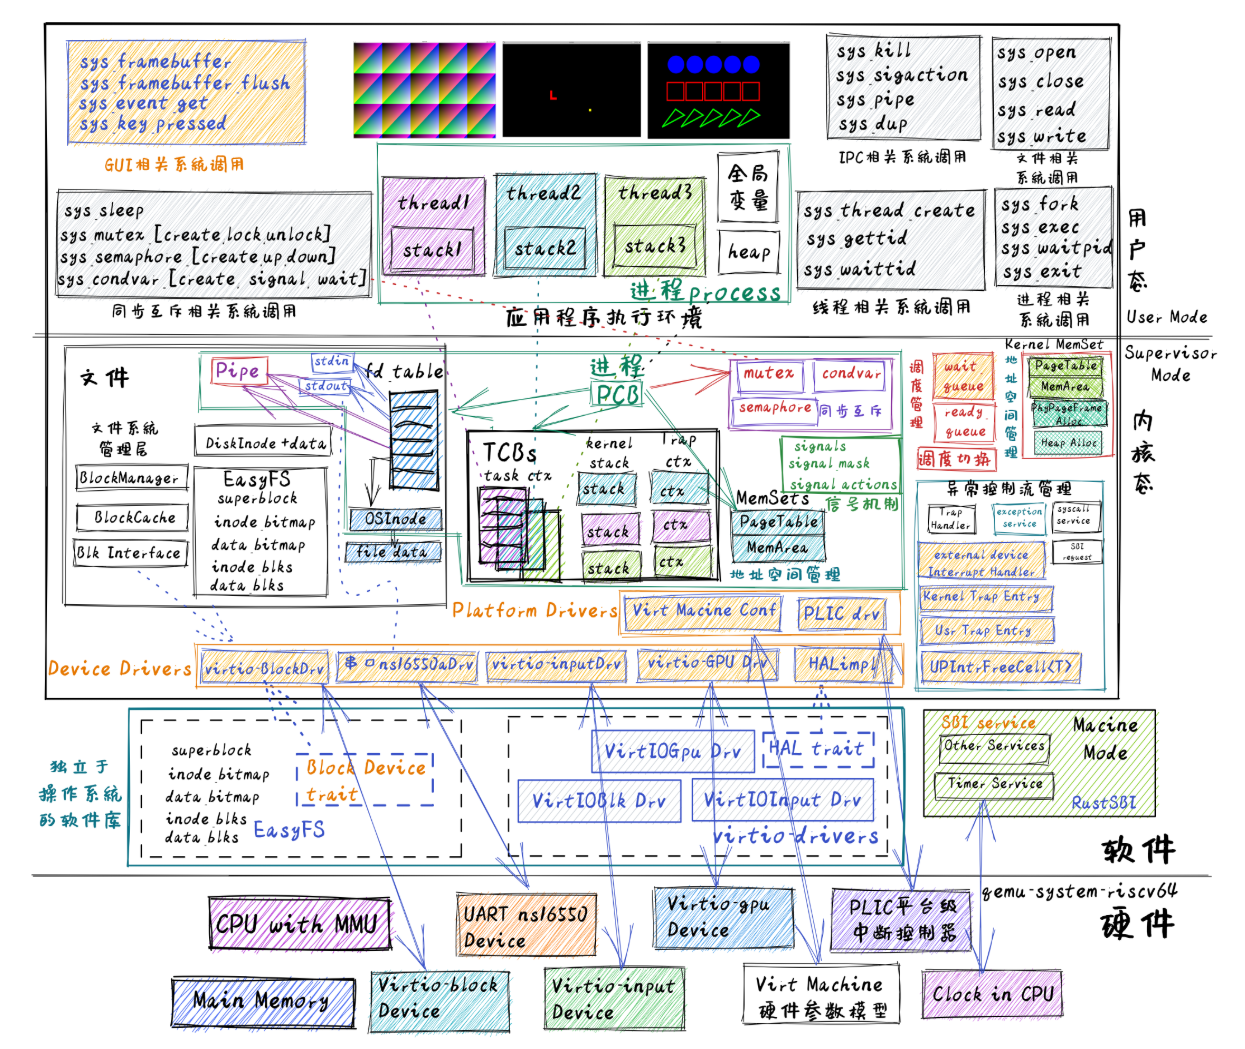
\includegraphics[width=1.0\textwidth]{../image/Architecture.png}
    \caption{系统架构图}
    \label{fig:architecture}
\end{figure}

% 第二章:系统启动与初始化
\chapter{系统启动与初始化}

我将本系统的启动与初始化分为三个阶段:

\begin{itemize}
    \item \textbf{QEMU初始化}
    \item \textbf{引导程序}
    \item \textbf{内核初始化}
\end{itemize}

\section{QEMU初始化}

这个阶段在真实计算机的启动中是加载ROM的过程。机器上电、文件加载到内存后,QEMU CPU的PC会被设置为0x1000,然后执行第一阶段的代码。
它会对CPU进行一些初始化操作,然后把控制权移交给bootloader,它的跳转地址固定是0x80000000处,我的BootLoader(rustsbi-qemu.bin)被预先加载到这里。

\section{引导程序}

在实际计算机中,Loader会进行内存初始化,并加载Runtime和BootLoader。BootLoader会进行硬件初始化和OS镜像的加载,而Runtime为OS提供运行时服务,
它是对硬件最基础的抽象,\href{https://github.com/riscv-non-isa/riscv-sbi-doc}{SBI}
就是RISC-V架构下的Runtime规范。

不过在NimlothOS中,引导程序和os镜像均在QEMU初始化阶段便已经被加载到了内存中,地址跳转以后直接进入rustsbi-qemu.bin程序,它会初始化硬件并提供SBI服务。

RustSBI的初始化结束以后,会跳转到预设好的0x80200000,这里放有内核镜像。

\section{内核初始化}

第三阶段是内核控制下操作系统各个模块的初始化,内核的入口函数是\lstinline[language=Rust]{rust_main},
它会在内核初始化完成后进入主循环调度。

\begin{lstlisting}[language=Rust,caption={内核初始化}, label={lst:kernel-init}]
#[unsafe(no_mangle)]
pub fn rust_main() -> ! {
    clear_bss();
    log::init();
    ::log::info!("[kernel] Hello, world!");
    mm::init();
    trap::init();
    trap::enable_timer_interrupt();
    timer::next_trigger();
    fs::list_apps();
    process::add_initproc();
    process::run_process();

    panic!("Unreachable in rust_main!");
}
\end{lstlisting}

下面进行详细介绍。

\subsection{内核镜像的内存分布}

默认链接器的内存布局是独立地址空间,但需要通过linker-qemu.ld脚本指定以符合QEMU的内存布局。调整后的具体布局如下:

\begin{figure}[htbp]
    \centering
    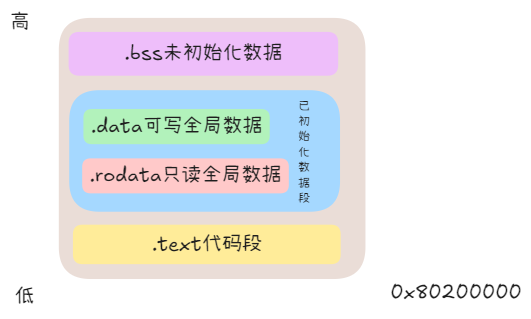
\includegraphics[width=0.6\textwidth]{../image/内核ELF布局.png}
    \caption{内核ELF布局}
    \label{fig:kernel-elf}
\end{figure}

通过 \texttt{rust-objdump} 工具查看编译后的内核镜像的各段分布与大小如下:

\begin{lstlisting}[language=Plain,caption={内核段分布信息}, label={lst:kernel-layout}]
$ rust-objdump -h target/riscv64gc-unknown-none-elf/release/os
target/riscv64gc-unknown-none-elf/release/os:   file format elf64-littleriscv
Sections:
Idx Name              Size     VMA              Type
1   .text             000178d0 0000000080200000 TEXT
2   .rodata           00005988 0000000080218000 DATA
3   .data             00000010 000000008021e000 DATA
4   .bss              00310330 000000008021f000 BSS
\end{lstlisting}

\subsection{汇编入口}

内核启动时的真正入口是一段汇编代码。在此之前,entry.asm会进行一些准备工作。它定义了内核入口函数\lstinline[language=Rust]{_start},
并把它放到.text的最低处(也即0x80200000处),另外在bss段建立大小64KB的内核启动栈。

运行时,\lstinline[language=Rust]{_start}会设置栈指针sp到栈顶并调用\lstinline[language=Rust]{rust_main},
然后过渡到\lstinline[language=Rust]{rust_main}代码中按顺序进行初始化。

\subsection{BSS段清零}

BSS段保护程序中未初始化的全局变量和静态变量,在程序加载过程中,它们需要被初始化为零。NimlothOS会利用链接文件里的符号sbss和ebss对这段
进行逐字节的清理。

\begin{lstlisting}[language=Rust,caption={bss段清零}, label={lst:bss-clear}]
fn clear_bss() {
    unsafe extern "C" {
        fn sbss();
        fn ebss();
    }
    unsafe {
        core::slice::from_raw_parts_mut(sbss as usize as *mut u8, ebss as usize - sbss as usize)
            .fill(0);
    }
}
\end{lstlisting}

\subsection{日志系统初始化}
日志系统在开发初期内置于内核中,现在正在尝试通过后期实现的管道机制将它从内核中抽离出来。内核中的日志系统基于Rust的log库实现
了Log trait,它的初始化工作是注册全局记录器并设置日志级别。

\subsection{内存系统初始化}
内存系统初始化的任务是按正确的顺序初始化内存管理的各个组件,确保系统能正常地进行内存分配和虚拟地址转化。
它会依次进行堆分配器初始化,物理页帧分配器初始化,并启用虚拟内存管理。

\begin{lstlisting}[language=Rust,caption={内存系统初始化}, label={lst:memory-init}]
pub fn init() {
    heap_allocator::init_heap();
    frame_allocator::init_frame_allocator();
    KERNEL_SPACE.exclusive_access().activate();
}
\end{lstlisting}

首先需要进行堆分配器的初始化,将静态分配的内核堆空间注册到堆分配器中,以便其可以用于动态内存分配。
这块空间位于前面提到的.bss段中,会一起被清零。

\begin{lstlisting}[language=Rust,caption={内核堆空间}, label={lst:heap-space}]
static mut HEAP_SPACE: [u8; KERNEL_HEAP_SIZE] = [0; KERNEL_HEAP_SIZE];
\end{lstlisting}

然后进行全局页帧分配器的初始化,设置它可用的物理内存范围。这里使用链接器脚本中定义的内核镜像的结束位置ekernel
作为可用物理内存的起点,终点通过硬编码到0x81000000,这样从0x80000000开始,可使用内存的整体大小为16MB。

\begin{lstlisting}[language=Rust,caption={物理页帧分配器初始化}, label={lst:frame-allocator-init}]
pub const MEMORY_END: usize = 0x8100_0000;

pub fn init_frame_allocator() {
    unsafe extern "C" {
        fn ekernel();
    }
    FRAME_ALLOCATOR.exclusive_access().init(
        PhysAddr::from(ekernel as usize).ceil(),
        PhysAddr::from(MEMORY_END).floor(),
    );
}
\end{lstlisting}

init会初始化一个简单的栈式页帧分配器StackFrameAllocator,其中的ceil和floor分别向上对齐和向下对齐到页边界。

最后,创建内核地址空间,并修改satp寄存器的值,启用SV39分页模式。我们的内核地址空间与xv6一样使用恒等映射,这样在
地址转化激活前后可以最大程度减少工作量。

\begin{lstlisting}[language=Rust,caption={内核地址空间激活}, label={lst:kernel-space-activate}]
pub fn activate(&self) {
    let satp = self.page_table.token();
    unsafe {
        satp::write(satp);
        asm!("sfence.vma");
    }
}
\end{lstlisting}

token函数根据页表的根节点计算出satp寄存器的值,然后通过asm!宏调用汇编指令写入satp寄存器,并执行sfence.vma指令,
刷新TLB缓存。

\begin{lstlisting}[language=Rust,caption={内核地址空间初始化}, label={lst:kernel-space-init}]
pub fn new_kernel() -> Self {
    let mut memory_set = Self::new_bare();
    memory_set.map_trampoline();
    println!(".text [{:#x}, {:#x})", stext as usize, etext as usize);
    println!(".rodata [{:#x}, {:#x})", srodata as usize, erodata as usize);
    println!(".data [{:#x}, {:#x})", sdata as usize, edata as usize);
    println!(
        ".bss [{:#x}, {:#x})",
        sbss_with_stack as usize, ebss as usize
    );
    println!("mapping .text section");
    memory_set.push(
        MapArea::new(
            (stext as usize).into(),
            (etext as usize).into(),
            MapType::Identical,
            MapPermission::R | MapPermission::X,
        ),
        None,
    );
    println!("mapping .rodata section");
    memory_set.push(
        MapArea::new(
            (srodata as usize).into(),
            (erodata as usize).into(),
            MapType::Identical,
            MapPermission::R,
        ),
        None,
    );
    println!("mapping .data section");
    memory_set.push(
        MapArea::new(
            (sdata as usize).into(),
            (edata as usize).into(),
            MapType::Identical,
            MapPermission::R | MapPermission::W,
        ),
        None,
    );
    println!("mapping .bss section");
    memory_set.push(
        MapArea::new(
            (sbss_with_stack as usize).into(),
            (ebss as usize).into(),
            MapType::Identical,
            MapPermission::R | MapPermission::W,
        ),
        None,
    );
    println!("mapping physical memory");
    memory_set.push(
        MapArea::new(
            (ekernel as usize).into(),
            MEMORY_END.into(),
            MapType::Identical,
            MapPermission::R | MapPermission::W,
        ),
        None,
    );
    println!("mapping memory-mapped registers");
    for pair in MMIO {
        memory_set.push(
            MapArea::new(
                (*pair).0.into(),
                ((*pair).0 + (*pair).1).into(),
                MapType::Identical,
                MapPermission::R | MapPermission::W,
            ),
            None,
        );
    }
    memory_set
}
\end{lstlisting}

\subsection{陷阱处理系统初始化与时钟中断设置}

陷阱处理系统与任务调度、信号处理等模块都有关,它的初始化只需要设置内核态陷阱入口,
用户态陷阱入口会在任务切换时的trap\_return中调用。内核态陷阱指向处理函数trap\_from\_kernel,
该函数输出陷阱相关寄存器后直接panic。

\begin{lstlisting}[language=Rust,caption={陷阱处理系统初始化与时钟中断设置}, label={lst:trap-timer-init}]
pub fn init() {
    set_kernel_trap_entry();
    enable_timer_interrupt();
}

pub fn next_trigger() {
    timer(time() + CLOCK_FREQ / TICKS_PER_SEC);
}
\end{lstlisting}

然后init函数还会启用时钟中断,设置sie\.STIE位,允许时钟中断触发陷阱。定时器和时钟模块也会调用
next\_trigger函数设置下一次时钟中断的触发时间。这也是进程调度系统的基础。

\subsection{文件系统初始化}
文件系统会调用list\_apps函数,在这个过程中惰性初始化的静态变量ROOT\_INODE,BLOCK\_DEVICE都会
进行加载,并调用文件系统的open函数来读取挂载到VirtIO块设备上的文件,恢复磁盘上这个文件系统的状态。

\begin{lstlisting}[language=Rust,caption={文件系统初始化}, label={lst:filesystem-init}]
lazy_static! {
    pub static ref ROOT_INODE: Arc<Inode> = {
        let efs = EasyFileSystem::open(BLOCK_DEVICE.clone());
        Arc::new(EasyFileSystem::root_inode(&efs))
    };
    pub static ref BLOCK_DEVICE: Arc<dyn BlockDevice> = {
        let block_device = Arc::new(BlockDeviceImpl::new());
        block_device
    };
}
\end{lstlisting}

\subsection{进程管理系统初始化}

到这里前期的初始化工作就正式完成了,内核将会把初始进程加入到就绪队列中,这一过程中同样通过惰性初始化机制
创建全局任务管理器PROCESS\_MANAGER和pid映射表PID\_MAP。

\begin{lstlisting}[language=Rust,caption={进程管理系统初始化}, label={lst:process-manager-init}]
lazy_static!{
    pub static ref PROCESS_MANAGER: UPSafeCell<TaskManager> =
        unsafe { UPSafeCell::new(ProcessManager::new()) };
    pub static ref PID2TCB: UPSafeCell<BTreeMap<usize, Arc<ProcessControlBlock>>> =
        unsafe { UPSafeCell::new(BTreeMap::new()) };
}
\end{lstlisting}

initproc是一个特殊的进程,它的pid为1。作为第一个用户进程,它会启动用户态入口,通过fork和exec系统调用
加载user\_shell程序,进入用户命令行解释器。

\subsection{进入主循环调度}

进程的调度由系统的idle控制流完成,它运行在CPU核的启动栈上,永不返回,并且对于进程而言是透明的。
这一机制由run\_process和schedule函数合作实现。

在内核初始化完毕后,就会调用run\_process函数进入idle控制流。它会从全局进程管理器获取下一个待调度进程
并切换。进程主动调用yield系统调用退出或是本轮时间耗尽触发中断时,会调用schedule函数回到idle控制流中进行
下一步调度。

\begin{lstlisting}[language=Rust,caption={idle控制流}, label={lst:idle-control-flow}]
pub fn run_process() {
    loop {
        let mut processor = PROCESSOR.exclusive_access();
        if let Some(process) = fetch_process() {
            let idle_process_cx_ptr = processor.idle_process_cx_ptr();
            let mut process_inner = process.inner_exclusive_access();
            let next_process_cx_ptr = &process_inner.process_cx as *const ProcessContext;
            process_inner.process_status = ProcessStatus::Running;
            drop(process_inner);
            processor.current = Some(process);
            drop(processor);
            unsafe {
                __switch(idle_process_cx_ptr, next_process_cx_ptr);
            }
        }
    }
}

pub fn schedule(switched_process_cx_ptr: *mut ProcessContext) {
    let mut processor = PROCESSOR.exclusive_access();
    let idle_process_cx_ptr = processor.idle_process_cx_ptr();
    drop(processor);
    unsafe {
        __switch(switched_process_cx_ptr, idle_process_cx_ptr);
    }
}
\end{lstlisting}

至此,系统的启动与初始化过程就全部完成了,可以通过user\_shell输入来运行用户程序。

\begin{figure}[htbp]
    \centering
    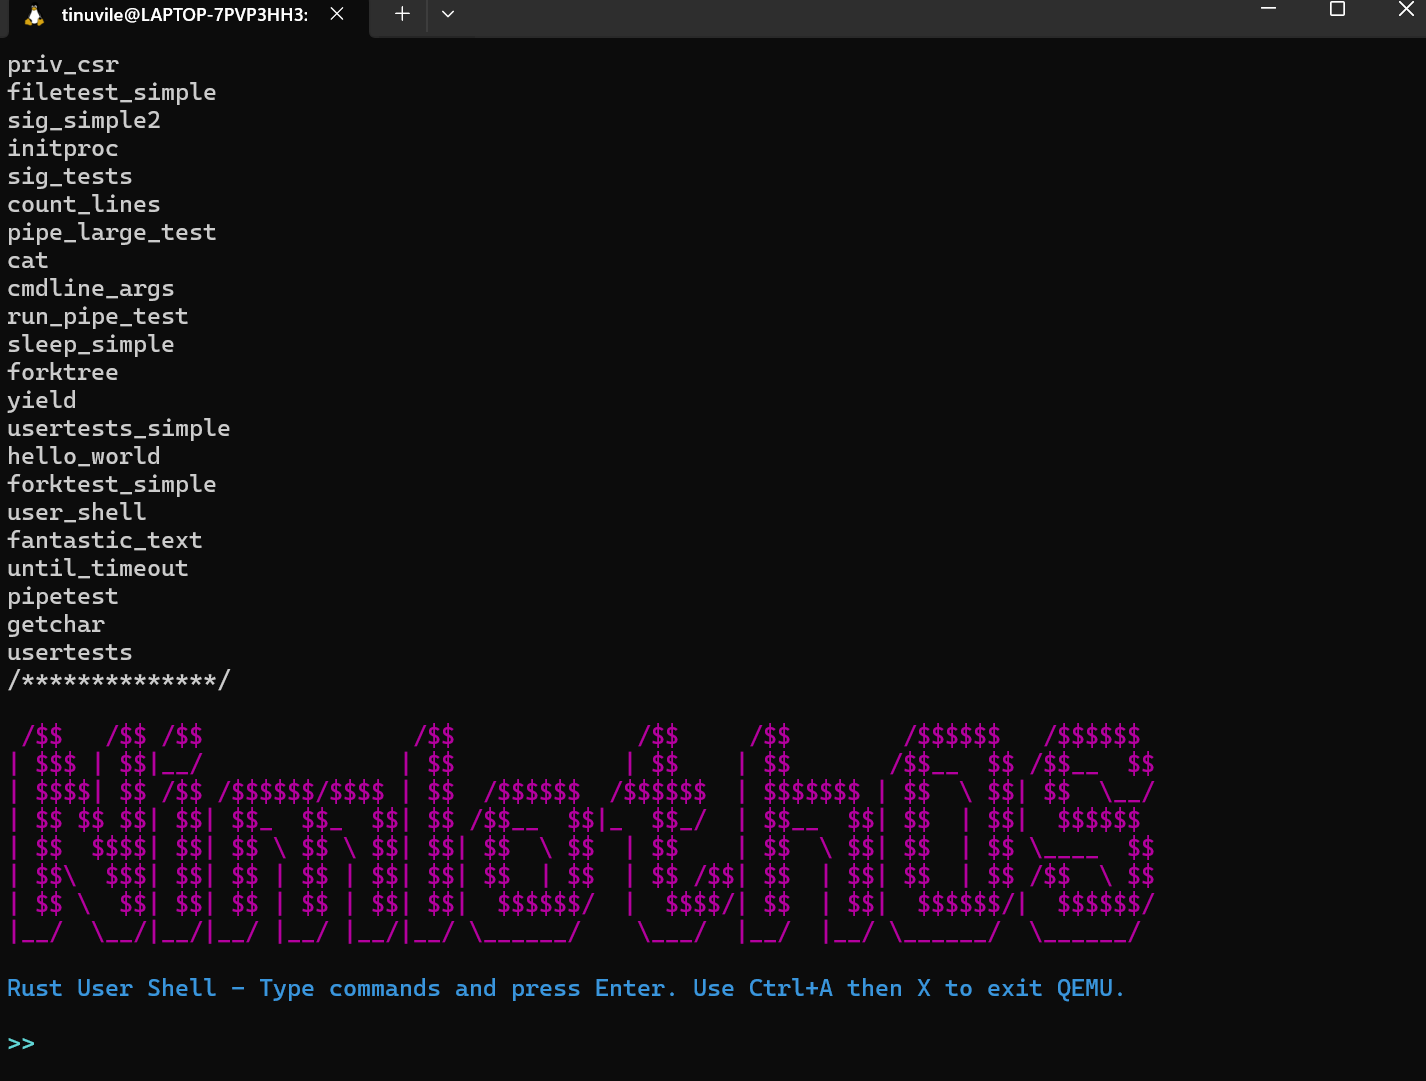
\includegraphics[width=0.6\textwidth]{../image/启动.png}
    \caption{启动}
    \label{fig:启动}
\end{figure}

% 第三章:内存管理系统
% \chapter{内存管理系统}

\section{系统设计}

NimlothOS的内存管理使用与xv6一样的\href{https://five-embeddev.com/riscv-priv-isa-manual/Priv-v1.12/supervisor.html#sec:sv39}{SV39}分页机制,
并实现了用户地址空间与内核地址空间分离。整体系统设计结构如下:

\begin{figure}[htbp]
    \centering
    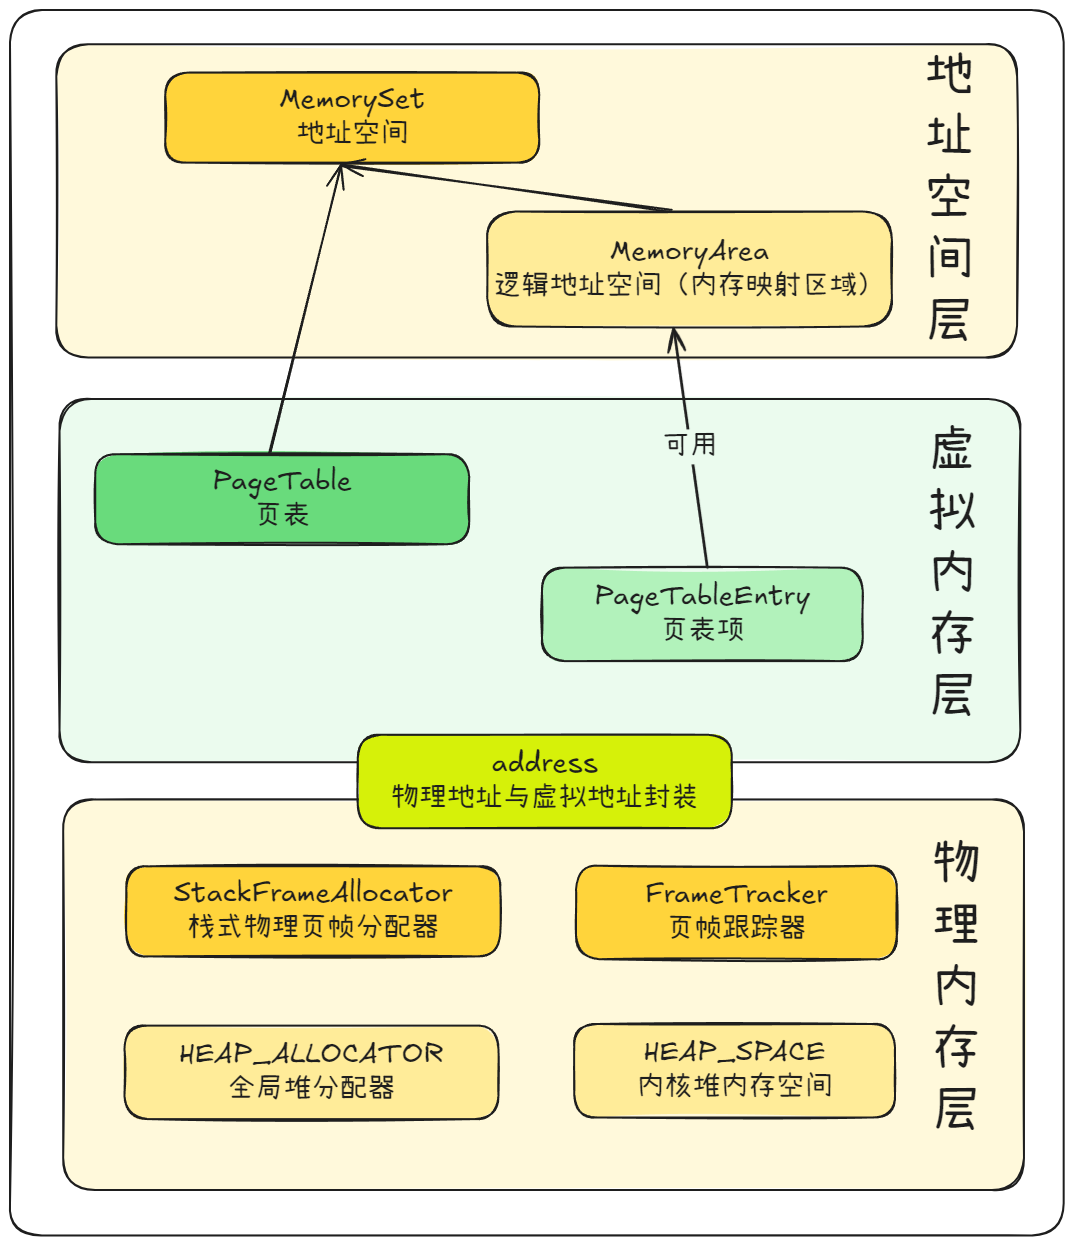
\includegraphics[width=0.4\textwidth]{../image/内存.png}
    \caption{内存系统结构}
    \label{fig:kernel-elf}
\end{figure}

\section{SV39}

Sv39的含义是它只用64bit虚拟地址的底部39位,剩下的25位不用,在这种配置中,RISC-V的页表在逻辑上是一个包含$2^{27}$个页表项的数组,每个页表项含一个44位的物理页号和一些标志位。
分页硬件通过使用39位中的顶部27位来索引页表以找到一个页表项,并生成一个56位的物理地址。物理地址的顶部44位来自页表项中的物理页号,底部12位从原始的虚拟地址中复制而来。

这里借用xv6 book中的图。

\begin{figure}[htbp]
    \centering
    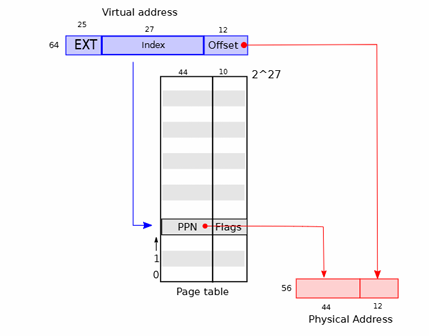
\includegraphics[width=0.4\textwidth]{../image/物理地址.png}
    \caption{物理地址}
    \label{fig:物理地址}
\end{figure}

\subsection{satp寄存器(Supervisor Address Translation and Protection Register)}

\href{https://five-embeddev.com/riscv-priv-isa-manual/Priv-v1.12/supervisor.html#sec:satp}{satp寄存器}用于控制管理模式下的地址转化与保护,其格式如下图:

\begin{figure}[htbp]
    \centering
    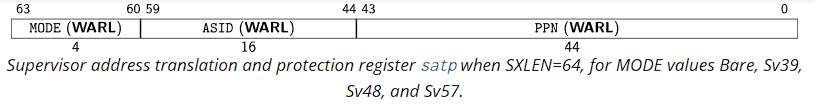
\includegraphics[width=0.8\textwidth]{../image/satp.png}
    \caption{satp寄存器}
    \label{fig:satp}
\end{figure}

当MODE没有设置时,虚拟地址即等于物理地址,当MODE设置时,就会启用分页模式,在此之后访存的地址必须
经过内存控制单元进行虚拟地址到物理地址的转换,再用它来访问物理内存。

\begin{figure}[htbp]
    \centering
    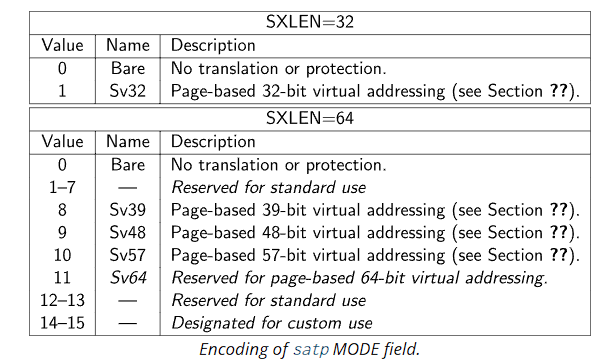
\includegraphics[width=0.6\textwidth]{../image/satpMode.png}
    \caption{satp mode字段的含义}
    \label{fig:satpMode}
\end{figure}

ASID字段用于性能优化,它可以区分不同进程的地址空间,但当前操作系统未实现,硬编码为0。如需地址空间切换时
会调用汇编命令\lstinline[language=Rust]{sfence.vma}来刷新TLB。

另外,satp寄存器的PPN处存放当前地址空间根页表的物理页号,satp的设置在内存管理系统初始化的时候完成,
此后地址空间切换也是调用汇编命令进行刷新\lstinline[language=Rust]{csrw satp, a1}。

\begin{lstlisting}[language=Rust,caption={satp设置}, label={lst:kernel-sections}]
pub fn activate(&self) {
    let satp = self.page_table.token();
    unsafe {
        satp::write(satp);
        asm!("sfence.vma");
    }
}
pub fn token(&self) -> usize {
    8usize << 60 | self.root_ppn.0
}
\end{lstlisting}

\subsection{地址格式}

\begin{figure}[htbp]
    \centering
    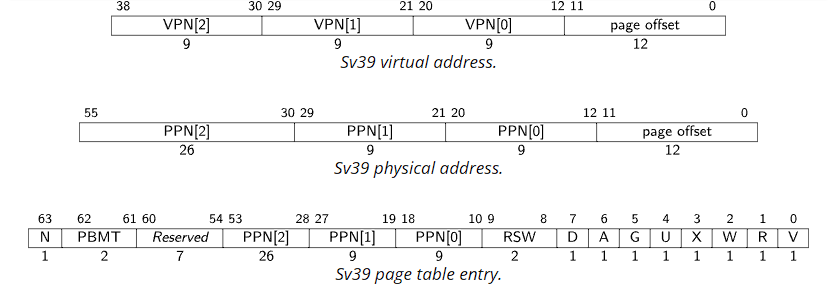
\includegraphics[width=0.8\textwidth]{../image/地址.png}
    \caption{地址与页表项}
    \label{fig:地址}
\end{figure}

虚拟地址和物理地址的低12位为页内偏移,这是因为设置单个页面大小为4KB。虚拟地址的高27位,可以看到分为L2、L1、L0,
它们是虚拟页号Virtual Page Number,物理地址的高44位同理。

页表项可以用虚拟页号为索引查到,它由物理页号和标志位组成。

值得注意的是,sv39规定\href{https://five-embeddev.com/riscv-priv-isa-manual/Priv-v1.12/supervisor.html#sec:sv39}{地址的63位到39位必须全部等于第38位},
否则将引发缺页异常。这意味着我们可以使用的地址空间只有高256G和低256G。

\subsection{地址转换}

地址转换过程中,首先会用虚拟页号的一级页索引去根页表中查二级页表的物理页号,
然后用虚拟页号的二级页索引去刚刚查到的二级页表中查三级页表的物理页号,
再用三级页索引在三级页表的物理页中查到物理页号,它与页内偏移拼接后就可得到物理地址。

\begin{figure}[htbp]
    \centering
    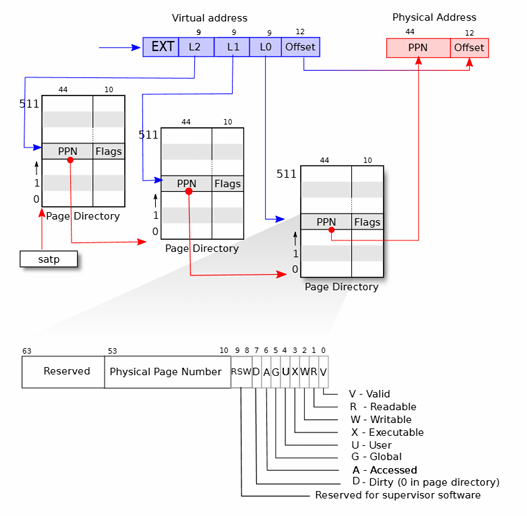
\includegraphics[width=0.7\textwidth]{../image/地址转换.png}
    \caption{地址转换}
    \label{fig:地址转换}
\end{figure}

\section{应用地址空间与内核地址空间}

NimlothOS实现了地址空间的隔离,每个应用都有自己的地址空间,内核地址空间与用户地址空间分离。

之前提到过SV39模式下规定地址的63位到39位必须全部等于第38位,否则将引发缺页异常。因此可用的
只有最高和最低的256GB,分别是第38位为0和为1的情况。

在内核地址空间中,os镜像的四个逻辑段和可分配物理内存的这段空间都是恒等映射,也即内核地址空间中,
0x80200000到0x81000000这段地址可以直接访问对应的物理空间,它们都在低256GB的区域。
其中,trampoline较为特殊,它既有一个直接映射,在text段中,同时又有一个单独映射,映射到内核地址空间的最高处。
内核地址空间高256GB的区域,则用于分配进程的内核栈,按照进程内核栈、保护页的顺序交替从TRAMPOLINE往下。
这部分就是帧映射了,它们会申请物理页帧,也即内核地址空间中ekernel到0x81000000这段区域,然后恒等映射到物理内存。
正是因为低地址区域全部采用恒等映射,内存系统初始化时不用担心MMU启用前后的切换问题。

应用地址空间中,从0x10000开始放置应用镜像的各个逻辑段,这定义在应用的链接器脚本中。在它的上面放置一个保护页,
然后分配用户栈,trampoline同样映射到地址最高的区域,同时在它的下面放置Trap上下文。

\begin{figure}[htbp]
    \centering
    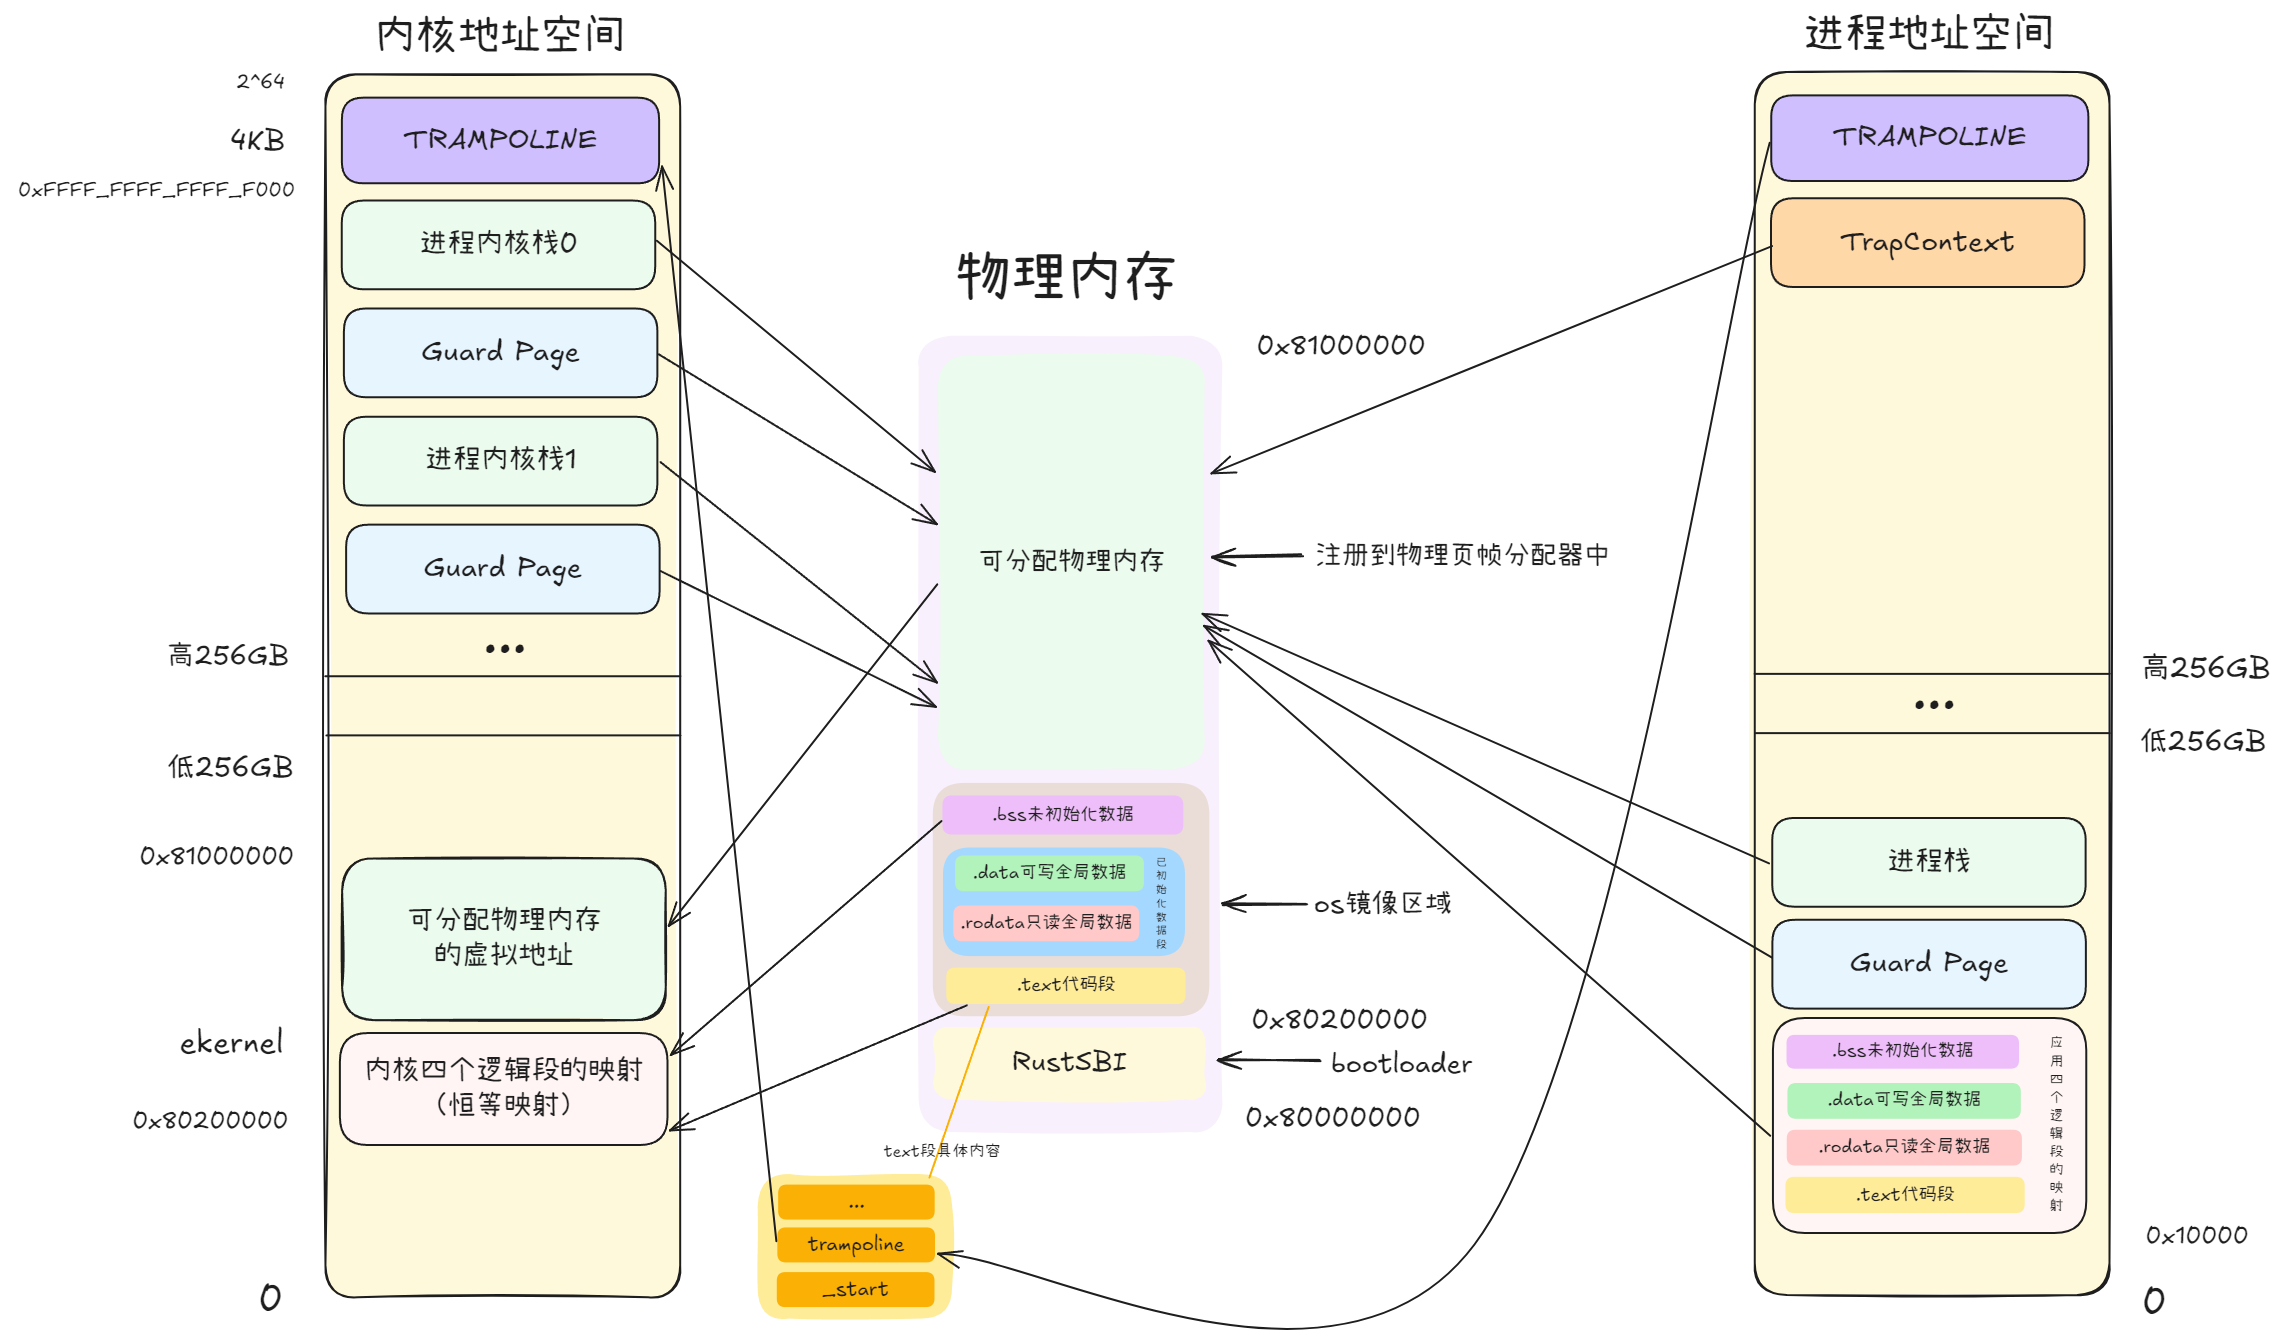
\includegraphics[width=1.0\textwidth]{../image/地址空间.png}
    \caption{地址空间}
    \label{fig:地址空间}
\end{figure}

\noindent
\rule{0.4\textwidth}{0.4pt}
\hfill
\text{以下为实现介绍}
\hfill
\rule{0.4\textwidth}{0.4pt}

\section{动态内存分配}

NimlothOS的内存管理包含两个层次的动态内存分配:堆分配器和物理页帧分配器。
堆分配器管理内核中的动态数据结构,而物理页帧分配器管理4KB大小的物理页面。

\subsection{堆分配器}

内存堆分配器负责管理内核中的动态数据结构,如向量、哈希表、字符串等。我用的是基于Buddy System算法实现的\lstinline[language=Rust]{buddy_system_allocator}库,
这种算法能够有效减少内存碎片,提供高效的动态内存管理。

系统预先为堆分配器保留了3MB的静态内存空间,该空间位于内核的BSS段中:

\begin{lstlisting}[language=Rust,caption={堆分配器声明}, label={lst:heap-decl}]
/// 全局堆分配器实例
#[global_allocator]
static HEAP_ALLOCATOR: LockedHeap<32> = LockedHeap::empty();

/// 内核堆内存空间(3MB)
static mut HEAP_SPACE: [u8; KERNEL_HEAP_SIZE] = [0; KERNEL_HEAP_SIZE];
\end{lstlisting}

\lstinline[language=Rust]{HEAP_ALLOCATOR}使用\lstinline[language=Rust]{#[global_allocator]}属性标记,使其成为Rust运行时使用的默认内存分配器。\lstinline[language=Rust]{LockedHeap<32>}中的32表示支持的最大分配块大小为$2^{32}$字节。

堆分配器的初始化过程相对简单,主要是将预分配的内存空间注册到分配器中:

\begin{lstlisting}[language=Rust,caption={堆分配器初始化}, label={lst:heap-init-func}]
pub fn init_heap() {
    unsafe {
        HEAP_ALLOCATOR
            .lock()
            .init(addr_of_mut!(HEAP_SPACE) as usize, KERNEL_HEAP_SIZE);
    }
}
\end{lstlisting}

初始化完成后,内核代码就可以使用标准的Rust内存分配接口,如\lstinline[language=Rust]{Vec::new()}、\lstinline[language=Rust]{Box::new()}等,这些操作会自动调用底层的Buddy System分配器。

\subsection{物理页帧分配器}

物理页帧分配器管理系统中所有的4KB物理页面,为页表、用户程序、内核数据结构等提供物理内存。NimlothOS采用栈式分配策略,这种策略既简单高效,又具有良好的内存局部性。

分配器的核心数据结构设计如下:

\begin{lstlisting}[language=Rust,caption={栈式页帧分配器结构}, label={lst:frame-allocator-struct}]
pub struct StackFrameAllocator {
    /// 下一个待分配的页号
    current: usize,
    /// 分配区间结束页号(不包含)
    end: usize,
    /// 回收页帧列表
    recycled: Vec<usize>,
}
\end{lstlisting}

分配器维护两种页帧来源:\lstinline[language=Rust]{current}到\lstinline[language=Rust]{end}的连续区间表示未使用的页帧,\lstinline[language=Rust]{recycled}向量存储已被释放可重复使用的页帧。

分配器的工作原理遵循以下策略:

\begin{itemize}
    \item \textbf{分配策略}:优先从回收列表弹出页帧(LIFO),这样可以提高缓存命中率
    \item \textbf{回收策略}:释放的页帧被推入回收列表,避免频繁的内存清零操作
    \item \textbf{RAII管理}:通过\lstinline[language=Rust]{FrameTracker}提供自动页帧释放,防止内存泄漏
\end{itemize}

页帧分配的实现体现了"先回收再新分配"的原则:

\begin{lstlisting}[language=Rust,caption={页帧分配逻辑}, label={lst:frame-alloc-logic}]
impl FrameAllocator for StackFrameAllocator {
    fn alloc(&mut self) -> Option<PhysPageNum> {
        if let Some(ppn) = self.recycled.pop() {
            // 优先使用回收的页帧
            Some(ppn.into())
        } else {
            // 回收列表为空时分配新页帧
            if self.current == self.end {
                None  // 内存耗尽
            } else {
                self.current += 1;
                Some((self.current - 1).into())
            }
        }
    }
}
\end{lstlisting}

页帧释放需要进行安全性检查,防止释放未分配的页帧:

\begin{lstlisting}[language=Rust,caption={页帧释放逻辑}, label={lst:frame-dealloc-logic}]
impl FrameAllocator for StackFrameAllocator {
    fn dealloc(&mut self, ppn: PhysPageNum) {
        let ppn = ppn.0;
        // 检查页帧是否已分配且未重复释放
        if ppn >= self.current || self.recycled.iter().find(|&v| *v == ppn).is_some() {
            panic!("Frame ppn={:#x} has not been allocated", ppn);
        }
        self.recycled.push(ppn);
    }
}
\end{lstlisting}

为了提供自动内存管理,系统实现了\lstinline[language=Rust]{FrameTracker},它利用Rust的RAII机制确保页帧的自动释放:

\begin{lstlisting}[language=Rust,caption={页帧跟踪器}, label={lst:frame-tracker}]
pub struct FrameTracker {
    pub ppn: PhysPageNum,
}

impl Drop for FrameTracker {
    fn drop(&mut self) {
        frame_dealloc(self.ppn);  // 自动释放页帧
    }
}
\end{lstlisting}

这样页帧的使用就变得非常安全,当\lstinline[language=Rust]{FrameTracker}超出作用域时,其包装的物理页帧会被自动释放,有效避免了内存泄漏问题。

系统在启动时会初始化页帧分配器,设置可分配的物理内存范围从内核镜像结束处\lstinline[language=Rust]{ekernel}到物理内存末尾\lstinline[language=Rust]{MEMORY_END}。

\section{地址抽象}

在实现页表管理之前,NimlothOS首先定义了一套地址抽象系统。

\subsection{地址类型系统}

NimlothOS定义了四个核心的地址类型,它们构成了内存管理的类型基础:

\begin{itemize}
    \item \textbf{PhysAddr}:物理地址,表示系统中的实际物理内存位置
    \item \textbf{VirtAddr}:虚拟地址,表示程序可见的地址空间位置  
    \item \textbf{PhysPageNum}:物理页号,表示4KB物理页面的编号
    \item \textbf{VirtPageNum}:虚拟页号,表示4KB虚拟页面的编号
\end{itemize}

\subsection{地址对齐与转换}

每种地址类型都提供了一些必要的操作方法。以物理地址为例,典型的有页对齐操作:

\begin{lstlisting}[language=Rust,caption={地址对齐操作}, label={lst:addr-align}]
impl PhysAddr {
    /// 向下对齐到页边界
    pub fn floor(&self) -> PhysPageNum {
        PhysPageNum(self.0 / PAGE_SIZE)
    }

    /// 向上对齐到页边界  
    pub fn ceil(&self) -> PhysPageNum {
        if self.0 == 0 {
            PhysPageNum(0)
        } else {
            PhysPageNum((self.0 - 1 + PAGE_SIZE) / PAGE_SIZE)
        }
    }
}
\end{lstlisting}

\lstinline[language=Rust]{floor()}方法将地址向下舍入到页边界,而\lstinline[language=Rust]{ceil()}方法则向上舍入。这些操作在内存分配时经常用到,确保分配的内存区域总是以页为单位。

\subsection{页面数据访问}

物理页号类型允许直接访问页面内容的能力,pte\_array返回包含512个页表项的可变切片,
方便对物理页中的内容进行修改。

\begin{lstlisting}[language=Rust,caption={页面访问接口}, label={lst:page-access}]
impl PhysPageNum {
    /// 将页面作为页表项数组访问
    pub fn pte_array(&self) -> &'static mut [PageTableEntry] {
        let pa: PhysAddr = self.clone().into();
        unsafe {
            core::slice::from_raw_parts_mut(
                pa.0 as *mut PageTableEntry,
                PAGE_SIZE / core::mem::size_of::<PageTableEntry>(),
            )
        }
    }

    /// 将页面作为字节数组访问
    pub fn bytes_array(&self) -> &'static mut [u8] {
        let pa: PhysAddr = self.clone().into();
        unsafe { 
            core::slice::from_raw_parts_mut(pa.0 as *mut u8, PAGE_SIZE) 
        }
    }
}
\end{lstlisting}

这些方法允许内核将物理页面按不同的数据结构来解释:当作页表时使用\lstinline[language=Rust]{pte_array()},当作普通数据存储时使用\lstinline[language=Rust]{bytes_array()}。

\subsection{虚拟页号的页表索引}

虚拟页号类型实现了索引计算:

\begin{lstlisting}[language=Rust,caption={页表索引计算}, label={lst:vpn-indexes}]
impl VirtPageNum {
    /// 获取三级页表索引
    pub fn indexes(&self) -> [usize; 3] {
        let mut vpn = self.0;
        let mut idx = [0usize; 3];
        for i in (0..3).rev() {
            idx[i] = vpn & 511;  // 取低9位
            vpn >>= 9;           // 右移9位
        }
        idx
    }
}
\end{lstlisting}

它将27位虚拟页号拆分为三个9位索引,分别用于访问三级页表的不同层级。这是实现SV39地址转换的关键步骤。

\section{页表管理}

页表是SV39分页机制的核心数据结构,负责将虚拟地址转换为物理地址。基于前面介绍的地址抽象系统,NimlothOS实现了三级页表结构管理。

\subsection{页表项结构}

每个页表项(Page Table Entry)占用8字节,按照RISC-V SV39规范,包含44位物理页号和8位标志位。使用\lstinline[language=Rust]{PageTableEntry}结构来封装这种底层的位操作,提供类型安全的接口。

页表项的基本结构定义如下:

\begin{lstlisting}[language=Rust,caption={页表项结构}, label={lst:pte-basic}]
pub struct PageTableEntry {
    /// 页表项的原始位表示  
    pub bits: usize,
}
\end{lstlisting}

\lstinline[language=Rust]{bits}字段直接存储页表项的64位原始数据,其中高44位为物理页号,低8位为标志位,中间12位保留。

页表项的创建需要指定目标物理页号和访问权限标志:

\begin{lstlisting}[language=Rust,caption={页表项创建}, label={lst:pte-create}]
impl PageTableEntry {
    pub fn new(ppn: PhysPageNum, flags: PTEFlags) -> Self {
        PageTableEntry {
            bits: ppn.0 << 10 | flags.bits() as usize,
        }
    }
}
\end{lstlisting}

物理页号左移10位放置到高位,标志位直接放置到低位,这样就构成了符合RISC-V规范的页表项格式。

页表项还提供了字段提取方法,用于获取其中包含的信息:

\begin{lstlisting}[language=Rust,caption={页表项字段提取}, label={lst:pte-extract}]
impl PageTableEntry {
    /// 获取物理页号
    pub fn ppn(&self) -> PhysPageNum {
        (self.bits >> 10 & ((1usize << 44) - 1)).into()
    }
    
    /// 检查页表项是否有效
    pub fn is_valid(&self) -> bool {
        (self.flags() & PTEFlags::V) != PTEFlags::empty()
    }
}
\end{lstlisting}

\lstinline[language=Rust]{ppn()}方法通过右移和掩码操作提取44位物理页号,而\lstinline[language=Rust]{is_valid()}方法检查V标志位来判断页表项是否有效。

页表项的标志位定义了内存页面的访问权限和状态信息,这些标志位的组合决定了页面的访问特性:

\begin{lstlisting}[language=Rust,caption={页表项标志位定义}, label={lst:pte-flags}]
bitflags! {
    pub struct PTEFlags: u8 {
        const V = 1 << 0;  // Valid - 页表项有效
        const R = 1 << 1;  // Readable - 可读
        const W = 1 << 2;  // Writable - 可写
        const X = 1 << 3;  // Executable - 可执行
        const U = 1 << 4;  // User accessible - 用户态可访问
        const G = 1 << 5;  // Global - 全局页面
        const A = 1 << 6;  // Accessed - 已访问
        const D = 1 << 7;  // Dirty - 已修改
    }
}
\end{lstlisting}

这些标志位的含义如下:
\begin{itemize}
    \item \textbf{V}:标示页表项是否有效,只有V=1的页表项才会被MMU处理
    \item \textbf{R/W/X}:分别控制读、写、执行权限,组合使用定义页面的访问特性
    \item \textbf{U}:控制用户态程序是否可以访问该页面
    \item \textbf{G}:标示该页面是全局页面,在地址空间切换时不会从TLB中清除
    \item \textbf{A/D}:由硬件自动设置,分别表示页面已被访问或修改
\end{itemize}

\subsection{页表结构}

\lstinline[language=Rust]{PageTable}结构是多级页表管理的核心,它不仅保存页表的根节点信息,还负责管理整个页表树的生命周期。

\begin{lstlisting}[language=Rust,caption={页表结构}, label={lst:page-table-struct}]
pub struct PageTable {
    /// 根页表的物理页号
    root_ppn: PhysPageNum,
    /// 页表页帧追踪器列表
    frames: Vec<FrameTracker>,
}
\end{lstlisting}

\lstinline[language=Rust]{root_ppn}存储根页表所在的物理页号,这个值会被写入satp寄存器来激活页表。\lstinline[language=Rust]{frames}向量管理所有页表页面的生命周期,确保页表页面在PageTable对象销毁时能够被正确回收。

页表最重要的功能是建立虚拟页号到物理页号的映射:

\begin{lstlisting}[language=Rust,caption={页面映射}, label={lst:page-map}]
impl PageTable {
    pub fn map(&mut self, vpn: VirtPageNum, ppn: PhysPageNum, flags: PTEFlags) {
        let pte = self.find_pte_create(vpn).unwrap();
        assert!(!pte.is_valid(), "vpn {:?} is mapped before mapping", vpn);
        *pte = PageTableEntry::new(ppn, flags | PTEFlags::V);
    }
}
\end{lstlisting}

\lstinline[language=Rust]{map()}方法首先通过\lstinline[language=Rust]{find_pte_create()}找到或创建目标虚拟页号对应的页表项,然后检查该页表项当前是否为空(防止重复映射),最后创建新的页表项建立映射关系。

取消映射的过程相对简单,只需要将页表项清空:

\begin{lstlisting}[language=Rust,caption={取消映射}, label={lst:page-unmap}]
impl PageTable {
    pub fn unmap(&mut self, vpn: VirtPageNum) {
        let pte = self.find_pte(vpn).unwrap();
        assert!(pte.is_valid(), "vpn {:?} is invalid before unmapping", vpn);
        *pte = PageTableEntry::empty();
    }
}
\end{lstlisting}

页表项查找是页表操作的核心算法,它实现了SV39的三级页表遍历:

\begin{lstlisting}[language=Rust,caption={页表项查找}, label={lst:find-pte}]
fn find_pte_create(&mut self, vpn: VirtPageNum) -> Option<&mut PageTableEntry> {
    let idxs = vpn.indexes();
    let mut ppn = self.root_ppn;
    let mut result: Option<&mut PageTableEntry> = None;
    
    for (i, idx) in idxs.iter().enumerate() {
        let pte = &mut ppn.pte_array()[*idx];
        if i == 2 {  // 到达叶子页表
            result = Some(pte);
            break;
        }
        if !pte.is_valid() {  // 需要创建中间页表
            let frame = frame_alloc().unwrap();
            *pte = PageTableEntry::new(frame.ppn, PTEFlags::V);
            self.frames.push(frame);
        }
        ppn = pte.ppn();  // 获取下级页表地址
    }
    result
}
\end{lstlisting}

该算法从根页表开始,逐级查找直到叶子页表。当遇到无效的中间页表项时,会自动分配新的物理页面来创建下级页表。
另外find\_pte函数同样实现了页表项的查找,但是它不会创建新的页表项,而是返回None。

\subsection{地址转换实现}

地址转换是页表管理的核心功能,它将虚拟地址空间映射到物理地址空间。NimlothOS提供了多个层次的转换接口。

最基础的转换是从虚拟页号到页表项:

\begin{lstlisting}[language=Rust,caption={虚拟页号转换}, label={lst:vpn-translate}]
impl PageTable {
    pub fn translate(&self, vpn: VirtPageNum) -> Option<PageTableEntry> {
        self.find_pte(vpn).map(|pte| *pte)
    }
}
\end{lstlisting}

该方法通过\lstinline[language=Rust]{find_pte()}查找页表项,如果找到有效页表项就返回其副本,否则返回None。
这样可以避免直接返回页表项引用可能带来的生命周期问题。

完整的虚拟地址到物理地址转换:

\begin{lstlisting}[language=Rust,caption={虚拟地址转换}, label={lst:va-translate}]
impl PageTable {
    pub fn translate_va(&self, va: VirtAddr) -> Option<PhysAddr> {
        self.find_pte(va.clone().floor()).map(|pte| {
            let aligned_pa: PhysAddr = pte.ppn().into();
            let offset = va.page_offset();
            let aligned_pa_usize: usize = aligned_pa.into();
            (aligned_pa_usize + offset).into()
        })
    }
}
\end{lstlisting}

该方法首先将虚拟地址向下对齐得到虚拟页号,然后查找对应的页表项获取物理页号,最后将物理页号转换为物理地址并加上页内偏移,
得到最终的物理地址。

页表还需要支持地址空间切换,这通过生成satp寄存器值来实现:

\begin{lstlisting}[language=Rust,caption={satp寄存器值生成}, label={lst:satp-token}]
impl PageTable {
    pub fn token(&self) -> usize {
        8usize << 60 | self.root_ppn.0
    }
}
\end{lstlisting}

该方法将SV39模式标识(8)左移到高位,与根页表物理页号组合,生成可以直接写入satp寄存器的值。当需要激活这个页表时,内核会将该值写入satp寄存器并刷新TLB。

\section{逻辑地址空间}

在实现了页表管理之后,需要进一步抽象出逻辑地址空间的概念。逻辑地址空间将连续的虚拟地址区间与特定的物理内存进行映射,每个区间都有自己的访问权限和映射方式。

\subsection{内存映射区域}

NimlothOS使用\lstinline[language=Rust]{MapArea}来表示一个连续的内存映射区域。每个映射区域包含虚拟地址范围、映射类型和访问权限等信息:

\begin{lstlisting}[language=Rust,caption={内存映射区域结构}, label={lst:map-area}]
pub struct MapArea {
    /// 虚拟地址区间
    vpn_range: VPNRange,
    /// 数据页面映射
    data_frames: BTreeMap<VirtPageNum, FrameTracker>,
    /// 映射类型
    map_type: MapType,
    /// 访问权限
    map_perm: MapPermission,
}
\end{lstlisting}

\lstinline[language=Rust]{vpn_range}定义了该区域覆盖的虚拟页号范围,\lstinline[language=Rust]{data_frames}是该设计的核心,它负责管理区域内每个虚拟页对应的物理页帧的生命周期。

映射类型定义了虚拟地址到物理地址的转换策略:

\begin{lstlisting}[language=Rust,caption={映射类型定义}, label={lst:map-type}]
pub enum MapType {
    /// 恒等映射:虚拟地址等于物理地址
    Identical,
    /// 分帧映射:每个虚拟页映射到独立的物理页帧
    Framed,
}
\end{lstlisting}

\lstinline[language=Rust]{Identical}映射主要用于内核地址空间,确保内核代码和数据的地址转换简单高效。\lstinline[language=Rust]{Framed}映射用于用户程序,提供了灵活的内存分配和保护机制。

访问权限控制了对内存区域的操作类型:

\begin{lstlisting}[language=Rust,caption={访问权限定义}, label={lst:map-permission}]
bitflags! {
    pub struct MapPermission: u8 {
        const R = 1 << 1;  // 可读
        const W = 1 << 2;  // 可写  
        const X = 1 << 3;  // 可执行
        const U = 1 << 4;  // 用户态可访问
    }
}
\end{lstlisting}

这些权限标志会在创建页表项时转换为相应的\lstinline[language=Rust]{PTEFlags},确保硬件MMU能够正确执行访问控制。

\subsection{映射区域操作}

基于前面介绍的生命周期管理机制,映射区域支持批量的映射和取消映射操作:

\begin{lstlisting}[language=Rust,caption={批量映射操作}, label={lst:map-area-batch}]
impl MapArea {
    /// 映射整个区域的所有页面
    pub fn map(&mut self, page_table: &mut PageTable) {
        for vpn in self.vpn_range {
            self.map_one(page_table, vpn);
        }
    }
    
    /// 取消映射整个区域的所有页面  
    pub fn unmap(&mut self, page_table: &mut PageTable) {
        for vpn in self.vpn_range {
            self.unmap_one(page_table, vpn);
        }
    }
}
\end{lstlisting}

这些批量操作方法内部调用了前面详细介绍的单页操作函数。通过这种设计,可以在创建地址空间时一次性建立所有必要的映射,在销毁时确保所有资源被正确清理。

\subsection{数据初始化}

对于包含初始数据的映射区域(如程序的代码段和数据段),需要将数据从外部存储加载到分配的物理页帧中:

\begin{lstlisting}[language=Rust,caption={映射区域数据复制}, label={lst:map-area-copy}]
impl MapArea {
    pub fn copy_data(&mut self, page_table: &mut PageTable, data: &[u8]) {
        assert_eq!(self.map_type, MapType::Framed);
        let mut start = 0usize;
        for vpn in self.vpn_range {
            let src = &data[start..start + PAGE_SIZE.min(data.len() - start)];
            let dst = &mut ppn.bytes_array()[..src.len()];
            dst.copy_from_slice(src);
            start += PAGE_SIZE;
            if start >= data.len() { break; }
        }
    }
}
\end{lstlisting}

这个方法按页面大小将数据分块复制到对应的物理页帧中,处理了数据大小不足一页的边界情况。

\subsection{物理页帧生命周期管理}

\lstinline[language=Rust]{data_frames}字段设计利用了RAII(Resource Acquisition Is Initialization)的思想。它使用\lstinline[language=Rust]{BTreeMap<VirtPageNum, FrameTracker>}数据结构来实现自动化的内存管理。

这样可以解决传统C语言内存管理中的几个核心问题:

\begin{itemize}
    \item \textbf{内存泄漏防护}:每个分配的物理页帧都有对应的\lstinline[language=Rust]{FrameTracker}负责自动释放
    \item \textbf{双重释放检测}:通过\lstinline[language=Rust]{BTreeMap}的唯一键约束防止同一页帧被多次释放  
    \item \textbf{异常安全性}:即使在系统异常时,析构函数也会确保资源正确回收
    \item \textbf{精确管理}:只管理\lstinline[language=Rust]{Framed}映射的页帧,\lstinline[language=Rust]{Identical}映射无需管理
\end{itemize}

\begin{lstlisting}[language=Rust,caption={页帧生命周期管理机制}, label={lst:frame-lifecycle}]
impl MapArea {
    // 页帧分配时的生命周期绑定
    pub fn map_one(&mut self, page_table: &mut PageTable, vpn: VirtPageNum) {
        let ppn = match self.map_type {
            MapType::Framed => {
                // 1. 分配新的物理页帧  
                let frame = frame_alloc().unwrap();
                let ppn = frame.ppn;
                
                // 2. 将FrameTracker绑定到虚拟页号
                // 此时页帧的所有权转移给MapArea管理
                self.data_frames.insert(vpn, frame);
                ppn
            },
            MapType::Identical => PhysPageNum(vpn.0),  // 无需管理
        };
        
        // 3. 在页表中建立映射关系
        let pte_flags = PTEFlags::from_bits(self.map_perm.bits).unwrap();
        page_table.map(vpn, ppn, pte_flags);
    }
    
    // 页帧释放时的自动清理
    pub fn unmap_one(&mut self, page_table: &mut PageTable, vpn: VirtPageNum) {
        if self.map_type == MapType::Framed {
            // 4. 从BTreeMap移除FrameTracker
            // 这里触发FrameTracker的Drop trait,自动释放页帧
            self.data_frames.remove(&vpn);
        }
        // 5. 清除页表映射
        page_table.unmap(vpn);
    }
}
\end{lstlisting}

它利用Rust的所有权系统实现了自动化的内存管理。当\lstinline[language=Rust]{FrameTracker}从\lstinline[language=Rust]{BTreeMap}中被移除时,它的\lstinline[language=Rust]{Drop}实现会被自动调用:

\begin{lstlisting}[language=Rust,caption={FrameTracker自动释放机制}, label={lst:frame-tracker-drop}]
impl Drop for FrameTracker {
    fn drop(&mut self) {
        // 自动将页帧返回给全局页帧分配器
        frame_dealloc(self.ppn);
    }
}
\end{lstlisting}

整个清理过程完全自动化:\lstinline[language=Rust]{MemorySet} → \lstinline[language=Rust]{MapArea} → \lstinline[language=Rust]{BTreeMap} → \lstinline[language=Rust]{FrameTracker} → 自动页帧释放。这种设计确保了即使在复杂的控制流程中(异常处理、panic等),物理内存也能被正确回收,极大提高了系统的健壮性。

\section{地址空间}

地址空间是逻辑地址空间的集合,代表了一个独立的虚拟内存环境。NimlothOS中每个进程都拥有自己的地址空间,内核也有独立的地址空间。

\subsection{地址空间结构}

\lstinline[language=Rust]{MemorySet}结构管理完整的地址空间,包含页表和所有的映射区域:

\begin{lstlisting}[language=Rust,caption={地址空间结构}, label={lst:memory-set}]
pub struct MemorySet {
    /// 多级页表
    page_table: PageTable,
    /// 映射区域集合
    areas: Vec<MapArea>,
}
\end{lstlisting}

\lstinline[language=Rust]{page_table}提供虚拟地址到物理地址的转换机制,\lstinline[language=Rust]{areas}向量管理所有的内存映射区域。这样可以将地址空间的不同部分(代码段、数据段、栈段等)统一管理。

地址空间提供了统一的映射接口,简化了区域管理:

\begin{lstlisting}[language=Rust,caption={地址空间映射操作}, label={lst:memory-set-ops}]
impl MemorySet {
    /// 插入新的映射区域
    pub fn push(&mut self, mut map_area: MapArea, data: Option<&[u8]>) {
        map_area.map(&mut self.page_table);
        if let Some(data) = data {
            map_area.copy_data(&mut self.page_table, data);
        }
        self.areas.push(map_area);
    }
    
    /// 激活地址空间
    pub fn activate(&self) {
        let satp = self.page_table.token();
        unsafe {
            satp::write(satp);
            asm!("sfence.vma");
        }
    }
}
\end{lstlisting}

\lstinline[language=Rust]{push()}方法将新的映射区域加入地址空间,并可选择性地初始化数据。\lstinline[language=Rust]{activate()}方法通过修改satp寄存器来切换到该地址空间,这是进程切换的关键步骤。

\subsection{内核地址空间}

内核地址空间是系统启动时创建的特殊地址空间,它使用恒等映射确保内核代码和数据的地址转换效率:

\begin{lstlisting}[language=Rust,caption={内核地址空间创建}, label={lst:kernel-memory-set}]
impl MemorySet {
    pub fn new_kernel() -> Self {
        let mut memory_set = Self::new_bare();
        
        // 映射内核各段
        memory_set.push(MapArea::new(
            (stext as usize).into(),
            (etext as usize).into(), 
            MapType::Identical,
            MapPermission::R | MapPermission::X,
        ), None);
        
        memory_set.push(MapArea::new(
            (srodata as usize).into(),
            (erodata as usize).into(),
            MapType::Identical, 
            MapPermission::R,
        ), None);
        
        memory_set.push(MapArea::new(
            (sdata as usize).into(),
            (edata as usize).into(),
            MapType::Identical,
            MapPermission::R | MapPermission::W,
        ), None);
        
        memory_set
    }
}
\end{lstlisting}

内核地址空间按照ELF段的权限要求进行映射:代码段具有读取和执行权限,只读数据段仅可读,可变数据段具有读写权限。

\subsection{用户地址空间}

用户地址空间的创建更加复杂,需要解析ELF文件并建立相应的映射关系:

\begin{lstlisting}[language=Rust,caption={用户地址空间创建}, label={lst:user-memory-set}]
impl MemorySet {
    pub fn from_elf(elf_data: &[u8]) -> (Self, usize, usize) {
        let mut memory_set = Self::new_bare();

        memory_set.map_trampoline();

        let elf = xmas_elf::ElfFile::new(elf_data).unwrap();
        let elf_header = elf.header;
        // elf.header.pt1:固定格式部分,pt2:可变格式部分
        let magic = elf_header.pt1.magic;
        assert_eq!(magic, [0x7f, 0x45, 0x4c, 0x46], "invalid elf!");
        let ph_count = elf_header.pt2.ph_count();
        let mut max_end_vpn = VirtPageNum(0);
        for i in 0..ph_count {
            let ph = elf.program_header(i).unwrap();
            if ph.get_type().unwrap() == xmas_elf::program::Type::Load {
                let start_va: VirtAddr = (ph.virtual_addr() as usize).into();
                let end_va: VirtAddr = ((ph.virtual_addr() + ph.mem_size()) as usize).into();
                let mut map_perm = MapPermission::U;
                let ph_flags = ph.flags();
                if ph_flags.is_read() {
                    map_perm |= MapPermission::R;
                }
                if ph_flags.is_write() {
                    map_perm |= MapPermission::W;
                }
                if ph_flags.is_execute() {
                    map_perm |= MapPermission::X;
                }
                let map_area = MapArea::new(start_va, end_va, MapType::Framed, map_perm);
                max_end_vpn = map_area.vpn_range.end();
                memory_set.push(
                    map_area,
                    Some(&elf.input[ph.offset() as usize..(ph.offset() + ph.file_size()) as usize]),
                );
            }
        }
        ...
    }
}
\end{lstlisting}

该方法解析ELF文件的程序头表,为每个可加载段创建对应的映射区域。通过检查段的标志位来设置正确的访问权限,并将段的数据加载到分配的物理页帧中。

\begin{lstlisting}[language=Rust,caption={用户栈映射}, label={lst:user-stack-map}]
    let max_end_va: VirtAddr = max_end_vpn.into();
    let mut user_stack_bottom: usize = max_end_va.into();
    // Guard Page
    user_stack_bottom += PAGE_SIZE;
    let user_stack_top: usize = user_stack_bottom + USER_STACK_SIZE;
    memory_set.push(
        MapArea::new(
            user_stack_bottom.into(),
            user_stack_top.into(),
            MapType::Framed,
            MapPermission::R | MapPermission::W | MapPermission::U,
        ),
        None,
    );
    // 堆空间的初始内存区域
    memory_set.push(
        MapArea::new(
            user_stack_top.into(),
            user_stack_top.into(),
            MapType::Framed,
            MapPermission::R | MapPermission::W | MapPermission::U,
        ),
        None,
    );
    // TrapContext
    memory_set.push(
        MapArea::new(
            TRAP_CONTEXT.into(),
            TRAMPOLINE.into(),
            MapType::Framed,
            MapPermission::R | MapPermission::W,
        ),
        None,
    );
    (
        memory_set,
        user_stack_top,
        elf.header.pt2.entry_point() as usize,
    )
\end{lstlisting}

用户地址空间还需要为用户栈分配空间,它中间隔有一个保护页。用户栈使用\lstinline[language=Rust]{Framed}映射,
具有读写权限,支持动态增长。

\subsection{地址空间切换}

地址空间切换是进程调度的核心操作,涉及页表的激活和TLB的刷新:

\begin{lstlisting}[language=Rust,caption={地址空间切换机制}, label={lst:address-space-switch}]
pub fn switch_address_space(new_memory_set: &MemorySet) {
    let old_satp = satp::read();
    let new_satp = new_memory_set.page_table.token();
    
    if old_satp != new_satp {
        unsafe {
            satp::write(new_satp);
            asm!("sfence.vma");
        }
    }
}
\end{lstlisting}

切换过程首先检查新旧地址空间是否相同,避免不必要的切换开销。当需要切换时,更新satp寄存器并执行\lstinline[language=Rust]{sfence.vma}指令刷新TLB,确保后续的地址转换使用新的页表。


% 第四章:任务管理与调度
% \include{chapters/ch04-task-scheduling}

% 第五章:中断与异常处理
% \chapter{中断与异常处理}

在操作系统运行中,有三种情况会导致CPU暂停普通指令的执行并强行将控制权转移给处理该事件的特殊代码:
第一种情况是系统调用,用户程序执行ecall指令请求内核为其执行某些操作时;
第二种情况是异常,当指令执行了非法操作时;
第三种情况是设备中断,当设备发出信号提示其需要注意时。
在NimlothOS中,这种情况统称为trap。操作系统对它们通常的处理流程是:

\begin{enumerate}
    \item trap强制将控制权转移到内核
    \item 内核保存寄存器和其他状态以便后续恢复执行
    \item 内核执行适当的处理程序代码
    \item 内核恢复保存的状态并从trap返回
\end{enumerate}

\section{系统设计}

正常情况下陷阱、中断与异常都是由内核的异常处理程序进行处理,它们对用户进程是不可见的,
NimlothOS中,实现了信号机制,使得进程可以得知发生的系统事件。信号机制是一种更高层次的软件形式的异常,
它同样会中断进程的控制流,可以由进程进行处理。因此在本系统中,陷阱处理机制与信号处理机制是紧密结合的。

目前实现的系统处理陷阱类型包括:

\begin{itemize}
    \item \textbf{系统调用}:用户程序通过ecall指令请求内核服务
    \item \textbf{时钟中断}:实现抢占式多进程调度的时间片机制
    \item \textbf{内存访问异常}:数据访问违规、页面错误等内存相关异常
    \item \textbf{指令异常}:非法指令、指令访问错误等执行异常
\end{itemize}

\section{陷阱处理相关硬件}

RISC-V架构为陷阱处理提供了完整的硬件支持,通过一系列控制状态寄存器(CSR)来管理陷阱的触发、处理和恢复过程。
NimlothOS充分利用了这些硬件机制,实现高效的陷阱处理系统。

\subsection{陷阱向量寄存器(stvec)}

\begin{figure}[htbp]
    \centering
    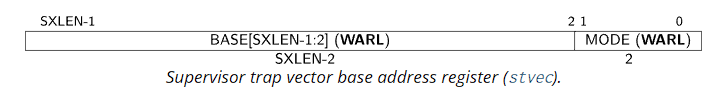
\includegraphics[width=1.0\textwidth]{../image/stvec.png}
    \caption{stvec寄存器}
    \label{fig:stvec}
\end{figure}

\href{https://five-embeddev.com/riscv-priv-isa-manual/Priv-v1.12/supervisor.html#supervisor-trap-vector-base-address-register-stvec}{stvec寄存器}
保存陷阱处理程序的入口地址,是陷阱处理的起始点。当陷阱发生时,硬件会自动将PC设置为stvec中存储的地址,
开始执行陷阱处理代码。

\begin{lstlisting}[language=Rust,caption={陷阱向量寄存器设置}, label={lst:stvec-setup}]
// 设置内核态陷阱入口
fn set_kernel_trap_entry() {
    unsafe {
        stvec::write(trap_from_kernel as usize, TrapMode::Direct);
    }
}
// 设置用户态陷阱入口  
fn set_user_trap_entry() {
    unsafe {
        stvec::write(TRAMPOLINE as usize, TrapMode::Direct);
    }
}
\end{lstlisting}

NimlothOS采用Direct模式,所有陷阱都跳转到同一个入口地址,然后由软件根据陷阱原因进行分发处理。

\subsection{陷阱原因寄存器(scause)}

\begin{figure}[htbp]
    \centering
    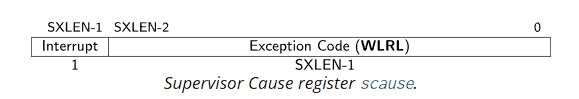
\includegraphics[width=0.8\textwidth]{../image/scause.png}
    \caption{scause寄存器}
    \label{fig:scause}
\end{figure}

\href{https://five-embeddev.com/riscv-priv-isa-manual/Priv-v1.12/supervisor.html#sec:scause}{scause寄存器}
记录了陷阱发生的原因,它的最高位是中断位,用于区分中断和异常,1表示中断,0表示异常,后面则是异常代码,标识具体的异常或中断类型。

scause寄存器的完整编码表如下:

\begin{table}[!htbp]
\centering
\caption{RISC-V陷阱原因编码表}
\label{tab:trap-causes}
\begin{tabular}{|c|c|l|}
\hline
\textbf{中断位} & \textbf{异常代码} & \textbf{描述} \\
\hline
\multicolumn{3}{|c|}{\textbf{中断类型 (Interrupt = 1)}} \\
\hline
1 & 0 & 保留 \\
1 & 1 & 监督者软件中断 \\
1 & 2–4 & 保留 \\
1 & 5 & \textbf{监督者时钟中断} \\
1 & 6–8 & 保留 \\
1 & 9 & 监督者外部中断 \\
1 & 10–15 & 保留 \\
1 & ≥16 & 平台专用 \\
\hline
\multicolumn{3}{|c|}{\textbf{异常类型 (Interrupt = 0)}} \\
\hline
0 & 0 & 指令地址未对齐 \\
0 & 1 & 指令访问错误 \\
0 & 2 & \textbf{非法指令} \\
0 & 3 & 断点 \\
0 & 4 & 加载地址未对齐 \\
0 & 5 & 加载访问错误 \\
0 & 6 & 存储/AMO地址未对齐 \\
0 & 7 & 存储/AMO访问错误 \\
0 & 8 & \textbf{用户态环境调用} \\
0 & 9 & 监督者态环境调用 \\
0 & 10–11 & 保留 \\
0 & 12 & 指令页面错误 \\
0 & 13 & \textbf{加载页面错误} \\
0 & 14 & 保留 \\
0 & 15 & \textbf{存储/AMO页面错误} \\
0 & 16–23 & 保留 \\
0 & 24–31 & 自定义使用 \\
0 & 32–47 & 保留 \\
0 & 48–63 & 自定义使用 \\
0 & ≥64 & 保留 \\
\hline
\end{tabular}
\end{table}

其中,NimlothOS当前处理的关键陷阱类型包括:

\begin{itemize}
    \item \textbf{异常代码5(中断)}:监督者时钟中断,用于实现抢占式调度
    \item \textbf{异常代码8}:用户态环境调用(ecall),对应系统调用
    \item \textbf{异常代码2}:非法指令异常,转换为SIGILL信号
    \item \textbf{异常代码13,15}:加载/存储页面错误,转换为SIGSEGV信号
    \item \textbf{异常代码1,5,7,12}:各种访问错误,转换为SIGSEGV信号
\end{itemize}

\subsection{陷阱值寄存器(stval)}

\begin{figure}[htbp]
    \centering
    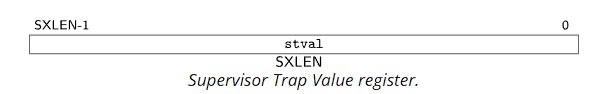
\includegraphics[width=0.7\textwidth]{../image/stval.png}
    \caption{stval寄存器}
    \label{fig:stval}
\end{figure}

\href{https://five-embeddev.com/riscv-priv-isa-manual/Priv-v1.12/supervisor.html#supervisor-trap-value-stval-register}{stval寄存器}提供陷阱相关的辅助信息:

\begin{itemize}
    \item \textbf{地址异常}:存储导致异常的虚拟地址
    \item \textbf{非法指令}:存储非法指令的编码
    \item \textbf{其他异常}:存储相关的错误信息
\end{itemize}

\subsection{监督者状态寄存器(sstatus)}

\begin{figure}[htbp]
    \centering
    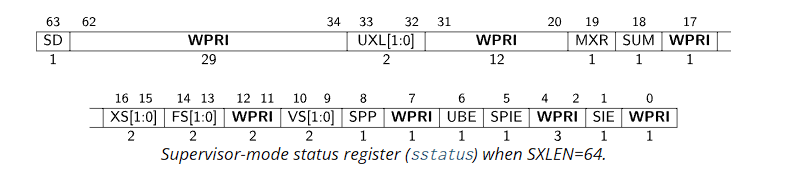
\includegraphics[width=0.8\textwidth]{../image/sstatus.png}
    \caption{sstatus寄存器}
    \label{fig:sstatus}
\end{figure}

\href{https://five-embeddev.com/riscv-priv-isa-manual/Priv-v1.12/supervisor.html#sstatus}{sstatus寄存器}控制处理器的状态和行为,
其中SPP位指示在进入管理模式前执行的特权级别,当发生陷阱时,如果陷阱来自用户态会设置为0,当执行sret指令时,会根据SSP位来恢复特权级别。
SIE位则用于在管理模式下启用或禁用所有中断,当SIE清零时,管理模式下不会接受中断;SPIE位指示在进入管理模式前是否启用了管理中断,当陷阱进入管理模式时,
SPIE位设置成SIE的值,SIE则清零,而执行sret指令时,SIE被设置成SPIE的值,SPIE清零。

\subsection{监督者异常程序计数器(sepc)}

\begin{figure}[htbp]
    \centering
    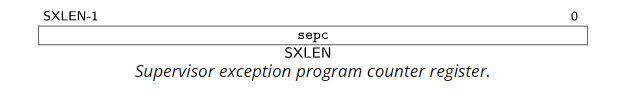
\includegraphics[width=0.7\textwidth]{../image/sepc.png}
    \caption{sepc寄存器}
    \label{fig:sepc}
\end{figure}

\href{https://five-embeddev.com/riscv-priv-isa-manual/Priv-v1.12/supervisor.html#supervisor-exception-program-counter-sepc}{sepc寄存器}
保存触发陷阱的指令地址,当执行sret指令时,sepc的值会被加载到PC寄存器,从而恢复到之前的特权级别。

\subsection{监督者暂存寄存器(sscratch)}

\begin{figure}[htbp]
    \centering
    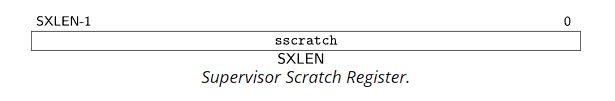
\includegraphics[width=0.7\textwidth]{../image/sscratch.png}
    \caption{sscratch寄存器}
    \label{fig:sscratch}
\end{figure}

\href{https://five-embeddev.com/riscv-priv-isa-manual/Priv-v1.12/supervisor.html#supervisor-scratch-register-sscratch}{sscratch寄存器}
用于在用户态和内核态之间切换时临时存储数据,当用户态执行时,存储陷阱上下文的地址,当陷阱处理时,与sp寄存器交换,实现栈切换。

\subsection{监督者中断使能寄存器(sie)}

\begin{figure}[htbp]
    \centering
    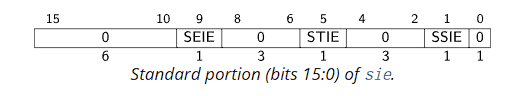
\includegraphics[width=0.7\textwidth]{../image/sie_.png}
    \caption{sie寄存器}
    \label{fig:sie}
\end{figure}

\href{https://five-embeddev.com/riscv-priv-isa-manual/Priv-v1.12/supervisor.html#supervisor-interrupt-registers-sip-and-sie}{sie寄存器}
控制各种中断的使能状态,每一位对应一种中断源:

\begin{itemize}
    \item \textbf{STIE}:时钟中断使能位
    \item \textbf{SEIE}:外部中断使能位  
    \item \textbf{SSIE}:软件中断使能位
\end{itemize}

\begin{lstlisting}[language=Rust,caption={中断使能设置}, label={lst:interrupt-enable}]
pub fn enable_timer_interrupt() {
    unsafe {
        sie::set_stimer(); // 启用时钟中断
    }
}
\end{lstlisting}

\subsection{硬件自动处理}

当陷阱发生时,RISC-V硬件会自动完成以下操作:

\begin{enumerate}
    \item \textbf{保存状态}:将当前特权级和中断状态保存到sstatus
    \item \textbf{记录原因}:将陷阱原因写入scause寄存器
    \item \textbf{保存地址}:将触发陷阱的指令地址保存到sepc
    \item \textbf{记录信息}:将相关信息(如出错地址)保存到stval
    \item \textbf{切换模式}:切换到监督者模式,禁用中断
    \item \textbf{跳转执行}:将PC设置为stvec中的地址开始执行
\end{enumerate}

\subsection{陷阱返回指令(sret)}

sret指令用于从监督者模式返回到之前的特权级,硬件会自动:

\begin{enumerate}
    \item \textbf{恢复PC}:将sepc的值加载到PC寄存器
    \item \textbf{恢复特权级}:根据sstatus.SPP恢复之前的特权级
    \item \textbf{恢复中断}:根据sstatus.SPIE恢复中断使能状态
    \item \textbf{清理状态}:清除sstatus.SPP,将SPIE复制到SIE
\end{enumerate}

\section{陷阱处理机制}

陷阱处理采用硬件与软件协同的方式。当陷阱发生时,RISC-V硬件自动完成特权级切换、
保存关键寄存器状态,然后跳转到内核设置的陷阱向量地址执行。
NimlothOS通过Trampoline页面和陷阱上下文结构,实现了完整的用户态状态保存与恢复机制。

\subsection{Trampoline}

Trampoline是一种地址空间切换机制。由于用户态发生陷阱时仍在用户地址空间中,
直接跳转到内核代码会导致地址转换错误。Trampoline页面同时映射到用户地址空间和内核地址空间的相同虚拟地址,
这样陷阱处理代码在地址空间切换的过程中能够正常找到trap.S放置在trampoline中的切换函数。

\subsection{处理流程}

陷阱处理的完整流程如下:

\begin{enumerate}
    \item \textbf{陷阱触发}:用户程序执行ecall指令或发生异常/中断
    \item \textbf{硬件切换}:CPU自动切换到S模式,跳转到stvec指定的处理程序
    \item \textbf{上下文保存}:\_\_alltraps保存所有寄存器到陷阱上下文
    \item \textbf{地址空间切换}:从用户地址空间切换到内核地址空间
    \item \textbf{处理分发}:trap\_handler根据陷阱类型执行相应处理
    \item \textbf{信号处理}:检查和处理进程待决信号
    \item \textbf{上下文恢复}:\_\_restore恢复寄存器并返回用户态
\end{enumerate}

\begin{figure}[!htbp]
    \centering
    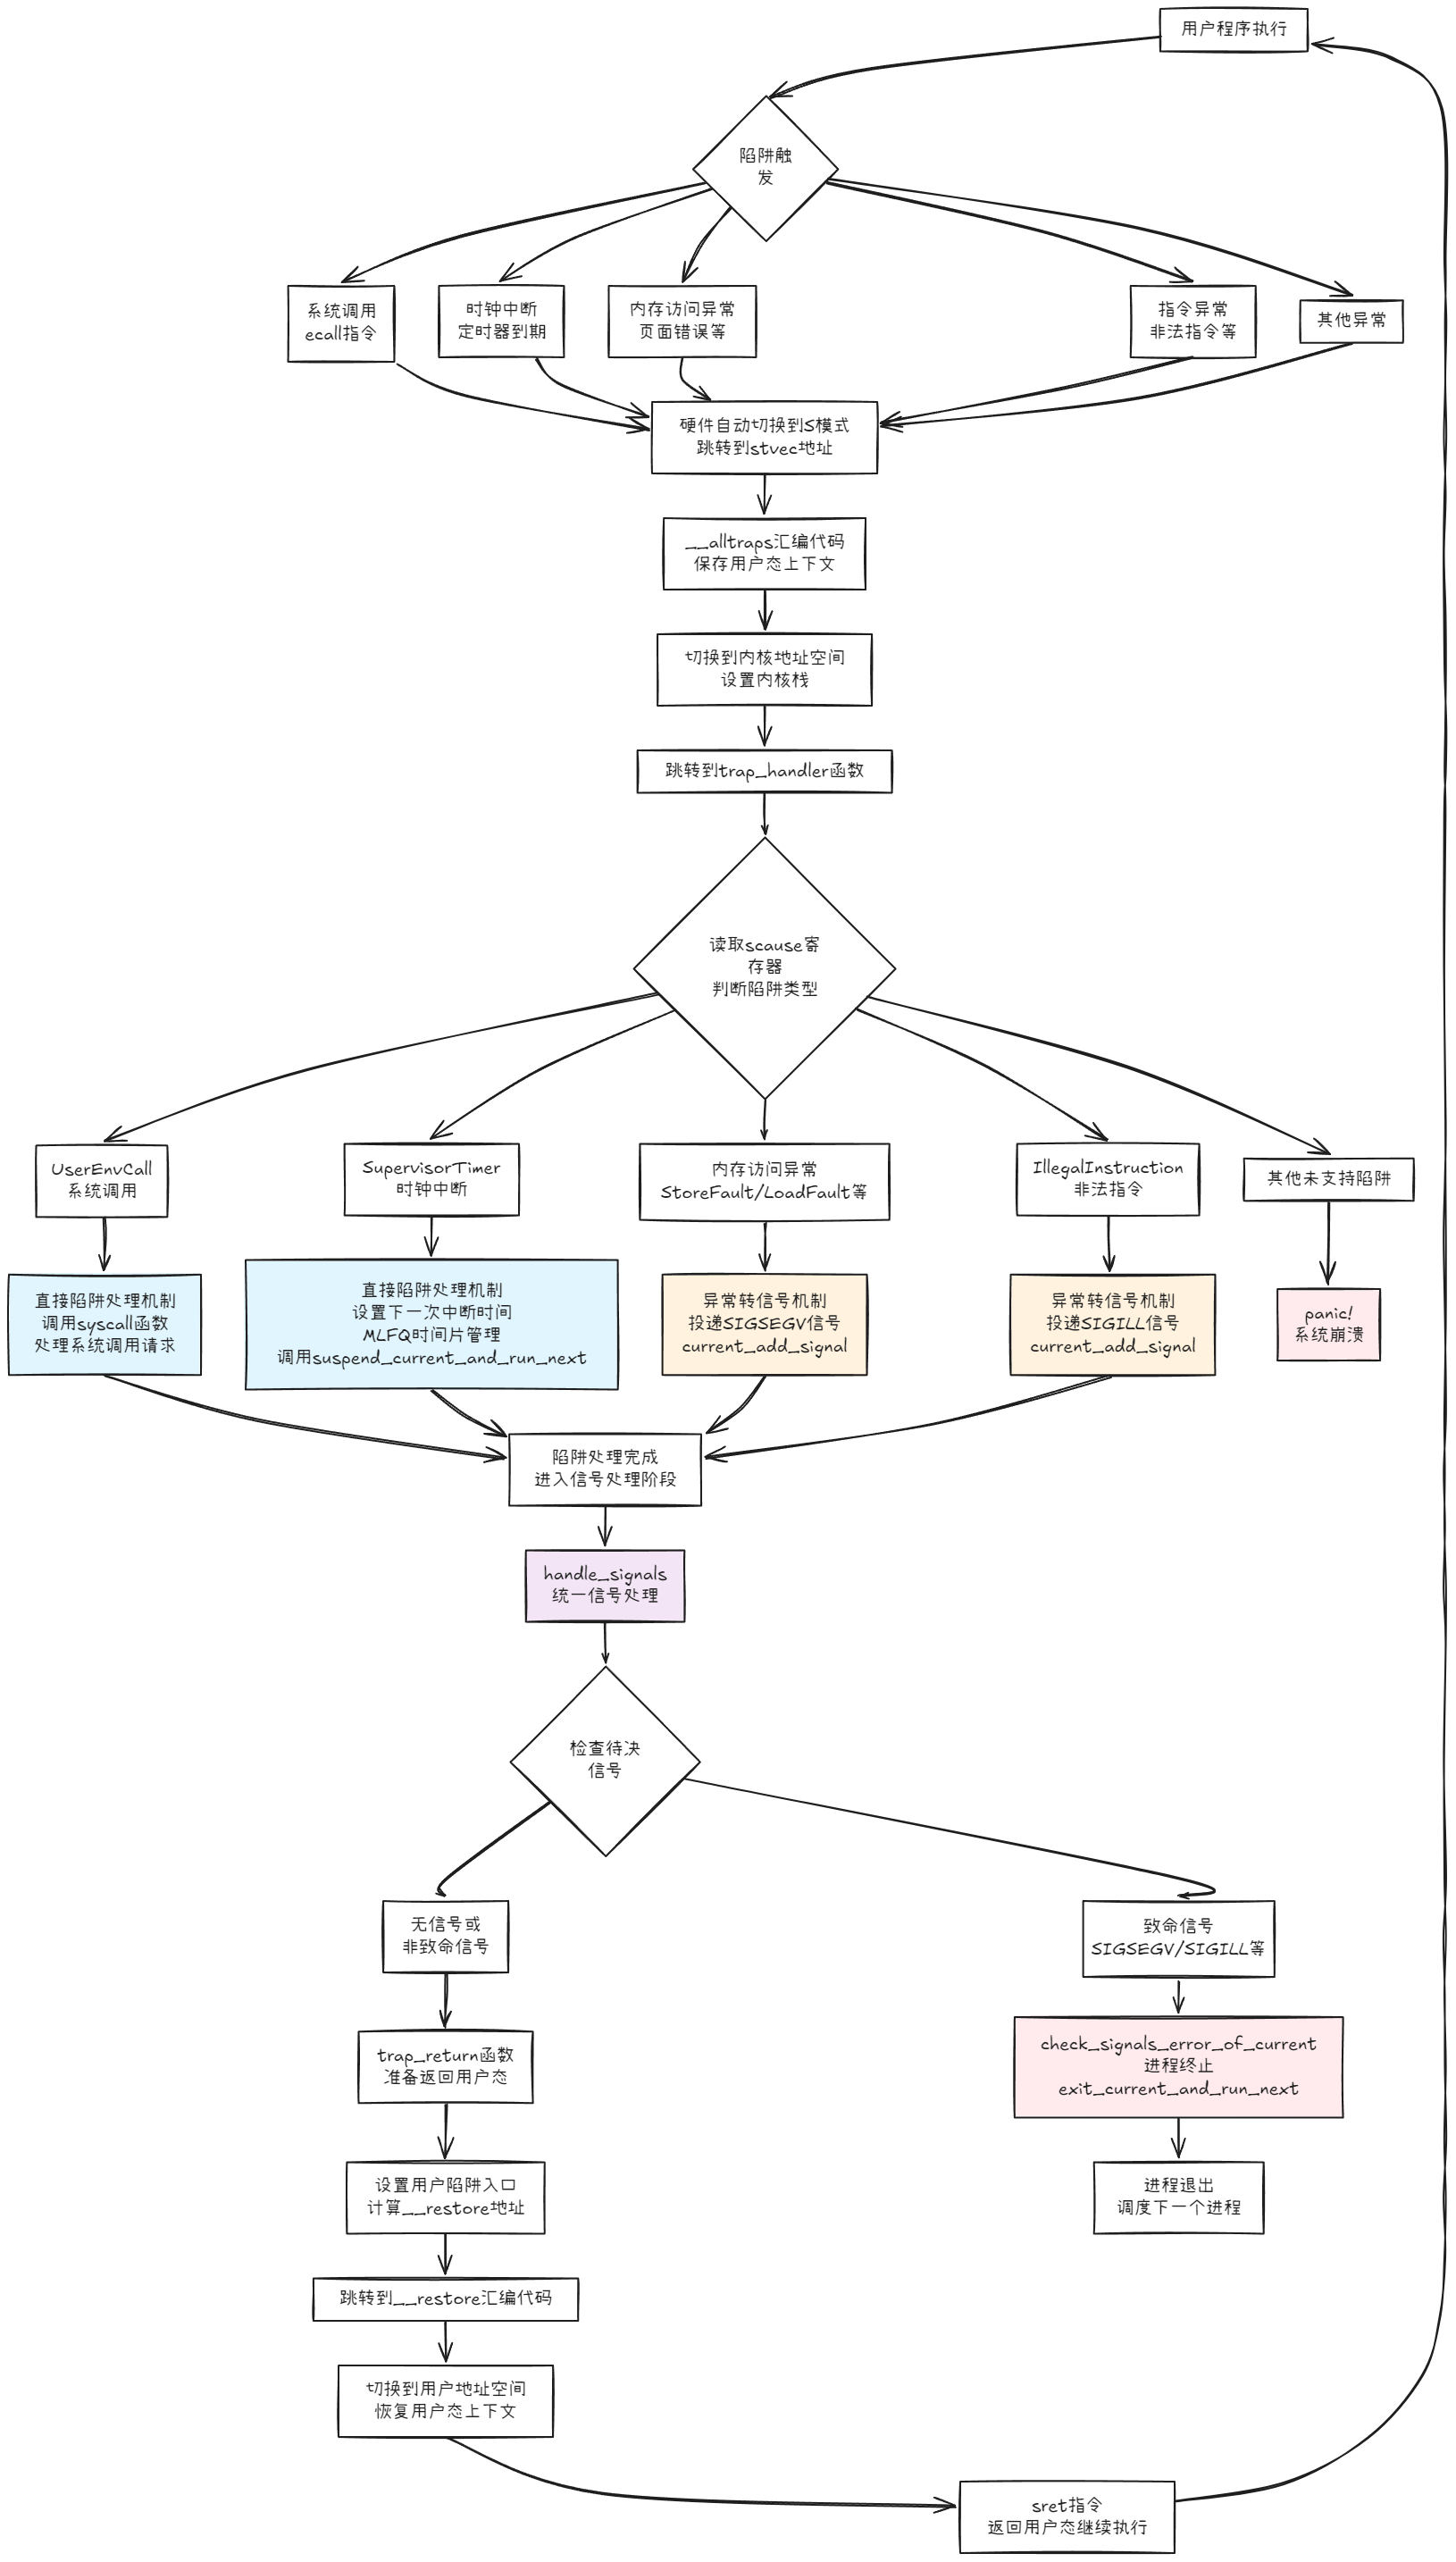
\includegraphics[width=0.8\textwidth]{../image/陷阱信号处理协作.png}
    \caption{陷阱处理流程}
    \label{fig:trap-process}
\end{figure}

\section{时钟中断与抢占调度}

时钟中断是实现抢占式多进程调度的关键机制。系统通过SBI接口设置定时器,
定期触发时钟中断,强制进行进程切换,确保没有进程能够无限期占用CPU资源。

在时钟中断处理中,NimlothOS实现了MLFQ调度算法的时间片管理:
每次中断都会增加当前进程的时间片使用计数,当达到该优先级队列的时间片限制时,
进程会被降级到下一个优先级队列,从而实现动态的优先级调整机制。

\noindent
\rule{0.4\textwidth}{0.4pt}
\hfill
\text{以下为实现介绍}
\hfill
\rule{0.4\textwidth}{0.4pt}

\section{陷阱上下文管理}

陷阱上下文是陷阱处理的核心数据结构,负责保存用户程序触发陷阱时的完整CPU状态。
与进程上下文不同,陷阱上下文需要保存所有寄存器,确保用户程序状态的完整性。

\subsection{陷阱上下文结构}

\begin{lstlisting}[language=Rust,caption={陷阱上下文结构}, label={lst:trap-context}]
#[repr(C)]
#[derive(Clone, Copy, Debug)]
pub struct TrapContext {
    /// 通用寄存器 x0-x31
    pub x: [usize; 32],
    /// 监督者状态寄存器 (sstatus)
    pub sstatus: Sstatus,
    /// 监督者异常程序计数器 (sepc)
    pub sepc: usize,
    /// 内核页表标识符
    pub kernel_satp: usize,
    /// 内核栈指针
    pub kernel_sp: usize,
    /// 陷阱处理函数地址
    pub trap_handler: usize,
}
\end{lstlisting}

陷阱上下文的设计考虑了陷阱处理的完整性和安全性需求。首先是\textbf{完整性保存},
系统保存所有32个通用寄存器,确保用户程序状态不丢失;其次是\textbf{特权级信息},
通过sstatus寄存器记录陷阱前的特权级和中断状态;再次是\textbf{返回地址},
sepc寄存器指向触发陷阱的指令地址,用于陷阱返回时恢复执行;最后是\textbf{内核环境准备},
kernel\_satp、kernel\_sp和trap\_handler三个字段为陷阱处理准备了完整的内核执行环境。

\subsection{上下文初始化}

系统为新创建的用户程序提供初始化陷阱上下文的功能:

\begin{lstlisting}[language=Rust,caption={陷阱上下文初始化}, label={lst:trap-context-init}]
impl TrapContext {
    pub fn app_init_context(
        entry: usize,
        sp: usize,
        kernel_satp: usize,
        kernel_sp: usize,
        trap_handler: usize,
    ) -> Self {
        let mut sstatus = sstatus::read();
        sstatus.set_spp(SPP::User); // 设置返回到用户态
        let mut cx = Self {
            x: [0; 32],
            sstatus,
            sepc: entry, // 设置程序入口地址
            kernel_satp,
            kernel_sp,
            trap_handler,
        };
        cx.sp(sp); // 设置用户栈指针
        cx
    }
}
\end{lstlisting}

初始化过程设置了程序入口地址、用户栈指针、返回特权级等关键信息,
确保用户程序能够在正确的环境中开始执行。

\section{陷阱处理核心}

陷阱处理的核心是trap\_handler函数,它作为所有用户态陷阱的统一入口,
负责分析陷阱类型并执行相应的处理逻辑。

\subsection{陷阱处理主函数}

\begin{lstlisting}[language=Rust,caption={陷阱处理主函数}, label={lst:trap-handler}]
#[unsafe(no_mangle)]
pub fn trap_handler() -> ! {
    set_kernel_trap_entry();
    let scause = scause::read();
    let stval = stval::read();
    match scause.cause() {
        Trap::Exception(Exception::UserEnvCall) => {
            let mut cx = current_trap_cx();
            cx.sepc += 4;
            let result = syscall(cx.x[17], [cx.x[10], cx.x[11], cx.x[12]]);
            cx = current_trap_cx();
            cx.x[10] = result as usize;
        }
        Trap::Exception(Exception::StoreFault)
        | Trap::Exception(Exception::StorePageFault)
        | Trap::Exception(Exception::LoadFault)
        | Trap::Exception(Exception::LoadPageFault)
        | Trap::Exception(Exception::InstructionFault)
        | Trap::Exception(Exception::InstructionPageFault) => {
            current_add_signal(SignalFlags::SIGSEGV);
        }
        Trap::Exception(Exception::IllegalInstruction) => {
            current_add_signal(SignalFlags::SIGILL);
        }
        Trap::Interrupt(Interrupt::SupervisorTimer) => {
            next_trigger();
            // MLFQ 时间片管理逻辑
            suspend_current_and_run_next();
        }
        _ => {
            panic!(
                "Unsupported trap {:?}, stval = {:#x}!",
                scause.cause(),
                stval,
            );
        }
    }

    handle_signals();
    if let Some((errno, msg)) = check_signals_error_of_current() {
        println!("[kernel] {}", msg);
        exit_current_and_run_next(errno);
    }
    trap_return();
}
\end{lstlisting}

\subsection{系统调用处理}

系统调用是用户程序请求内核服务的标准方式。在RISC-V架构中,用户程序通过ecall指令触发系统调用,
系统调用处理涉及多个关键环节。首先是\textbf{参数传递},系统调用号存储在x17寄存器,
而调用参数存储在x10-x12寄存器中;然后是\textbf{返回值处理},系统调用的返回值会写入x10寄存器供用户程序获取;
接下来是\textbf{PC调整},系统需要将sepc增加4来跳过ecall指令,避免陷阱返回后重复执行;
最后是\textbf{上下文管理},由于系统调用处理过程中可能发生进程调度,
因此需要两次获取陷阱上下文来处理可能出现的上下文变化。

\subsection{异常转信号机制}

NimlothOS采用"异常转信号"的方法,将传统的直接杀死进程改为投递信号。
对于\textbf{内存访问异常},系统将其转换为SIGSEGV信号;
对于\textbf{非法指令异常},系统将其转换为SIGILL信号;
这样允许用户程序自定义信号处理函数来应对异常情况;同时达到了\textbf{统一管理}的目标,
通过信号系统统一处理各种异常情况,实现更一致和可控的异常处理机制。

\section{时钟中断与调度}

时钟中断是实现抢占式调度的核心机制,它定期打断用户程序的执行,
给调度器一个重新分配CPU的机会。

\subsection{时钟中断初始化}

系统在启动时需要初始化时钟中断:

\begin{lstlisting}[language=Rust,caption={时钟中断初始化}, label={lst:timer-init}]
pub fn init() {
    set_kernel_trap_entry();
    enable_timer_interrupt();
}
pub fn enable_timer_interrupt() {
    unsafe {
        sie::set_stimer();
    }
}
\end{lstlisting}

\subsection{MLFQ时间片管理}

在时钟中断处理中,系统实现了MLFQ调度算法的时间片管理机制,这个在进程部分已经有过介绍,
这里不再赘述。

\section{底层汇编实现}

陷阱处理的底层切换使用汇编代码,负责寄存器的保存和恢复。

\subsection{陷阱保存机制}

\begin{lstlisting}[language={[x86masm]Assembler},caption={陷阱上下文保存}, label={lst:alltraps}]
__alltraps:
    # 交换 sscratch and sp(x2) 寄存器内容
    csrrw sp, sscratch, sp
    # 现在sp->kernel stack,sscratch->user stack
    # 保存通用寄存器,跳过x0,tp(x4)
    sd x1, 1*8(sp)
    sd x3, 3*8(sp)
    .set n, 5
    .rept 27
        SAVE_GP %n
        .set n, n+1
    .endr
    # 读寄存器并保存
    csrr t0, sstatus
    csrr t1, sepc
    sd t0, 32*8(sp)
    sd t1, 33*8(sp)
    # sscratch 现在指向用户栈
    csrr t2, sscratch
    sd t2, 2*8(sp)
    # 保存kernel_satp到t0
    ld t0, 34*8(sp)
    # 保存trap_handler到t1
    ld t1, 36*8(sp)
    # 跳转到kernel_sp
    ld sp, 35*8(sp)
    # 切换到内核地址空间
    csrw satp, t0
    sfence.vma
    # 跳转到trap_handler
    jr t1
\end{lstlisting}

保存过程按照严格的顺序执行五个关键步骤。首先进行\textbf{栈指针切换},
通过sscratch寄存器实现用户栈到内核栈的切换;接着进行\textbf{寄存器保存},
逐个保存所有通用寄存器到陷阱上下文中确保状态完整性;然后是\textbf{CSR保存},
保存sstatus和sepc等关键控制寄存器的状态信息;随后执行\textbf{地址空间切换},
更新satp寄存器将执行环境从用户地址空间切换到内核地址空间;
最后\textbf{跳转执行},跳转到trap\_handler函数开始内核态的陷阱处理流程。

\subsection{陷阱恢复机制}

\begin{lstlisting}[language={[x86masm]Assembler},caption={陷阱上下文恢复}, label={lst:restore}]
__restore:
    # 切换到用户地址空间
    csrw satp, a1
    sfence.vma
    csrw sscratch, a0
    mv sp, a0
    # 恢复CSR和通用寄存器
    ld t0, 32*8(sp)
    ld t1, 33*8(sp)
    csrw sstatus, t0
    csrw sepc, t1
    ld x1, 1*8(sp)
    ld x3, 3*8(sp)
    .set n, 5
    .rept 27
        LOAD_GP %n
        .set n, n+1
    .endr
    # 恢复用户栈指针
    ld sp, 2*8(sp)
    sret
\end{lstlisting}

恢复过程与保存过程相反,按照逆序执行五个步骤来完整恢复用户态执行环境。
首先进行\textbf{地址空间切换},将执行环境从内核地址空间切换回用户地址空间;
接着进行\textbf{CSR恢复},恢复sstatus和sepc等关键控制寄存器的状态;
然后执行\textbf{寄存器恢复},逐个恢复所有通用寄存器到用户程序被中断前的状态;
随后进行\textbf{栈指针恢复},将栈指针切换回用户程序的栈;
最后执行\textbf{返回用户态},通过sret指令完成特权级切换并跳转回用户程序继续执行。

\section{陷阱返回机制}

陷阱处理完成后,系统需要通过trap\_return函数安全地返回用户态。

\subsection{返回流程}

\begin{lstlisting}[language=Rust,caption={陷阱返回实现}, label={lst:trap-return}]
#[unsafe(no_mangle)]
pub fn trap_return() -> ! {
    set_user_trap_entry();
    let trap_cx_ptr = TRAP_CONTEXT;
    let user_satp = current_user_token();
    unsafe extern "C" {
        fn __alltraps();
        fn __restore();
    }
    let restore_va = __restore as usize - __alltraps as usize + TRAMPOLINE;
    unsafe {
        asm!(
            "fence.i",
            "jr {restore_va}",
            restore_va = in(reg) restore_va,
            in("a0") trap_cx_ptr,
            in("a1") user_satp,
            options(noreturn),
        );
    }
}
\end{lstlisting}

返回过程首先进行\textbf{用户陷阱入口设置},重新配置stvec寄存器指向Trampoline页面,
为后续可能的陷阱做好准备;接着\textbf{准备参数},将陷阱上下文地址和用户页表标识符
作为参数传递给恢复函数;然后执行\textbf{地址计算},计算\_\_restore函数在Trampoline中的正确虚拟地址;
最后进行\textbf{跳转恢复},通过内联汇编跳转到\_\_restore函数开始执行恢复过程。

\section{信号处理集成}

陷阱处理系统与信号处理机制紧密集成,每次陷阱处理完成后都会检查进程的待决信号:

\begin{lstlisting}[language=Rust,caption={信号处理集成}, label={lst:signal-integration}]
handle_signals();

if let Some((errno, msg)) = check_signals_error_of_current() {
    println!("[kernel] {}", msg);
    exit_current_and_run_next(errno);
}

trap_return();
\end{lstlisting}


% 第六章:系统调用接口
% \chapter{系统调用接口}

\section{系统设计}

系统调用接口是用户程序与操作系统内核交互的标准机制,它为用户程序访问系统服务提供了一套统一的API。
NimlothOS实现了完整的系统调用体系,支持文件操作、进程管理、信号处理等核心功能。

\subsection{调用约定}

NimlothOS遵循RISC-V架构的标准系统调用约定,使用\texttt{ecall}指令触发系统调用。
调用参数通过寄存器传递:系统调用号存储在\texttt{a7}寄存器,
参数按顺序存储在\texttt{a0}、\texttt{a1}、\texttt{a2}寄存器中,
返回值通过\texttt{a0}寄存器返回给用户程序。

\subsection{系统调用分类}

NimlothOS的系统调用按功能分为三大类:

\textbf{文件系统接口}提供了完整的文件I/O功能,包括文件的打开、关闭、读写操作,
以及管道通信机制,支持进程间的数据交换和重定向操作。

\textbf{进程管理接口}实现了完整的进程生命周期管理,支持进程创建、执行、等待和退出,
提供了fork-exec模型的完整实现,支持多进程并发执行和父子进程协作。

\textbf{信号处理接口}提供了异步事件处理机制,支持信号的发送、接收和自定义处理,
实现了类Unix的信号语义,为异常处理和进程间通信提供了支撑。

\subsection{安全机制}

系统调用的安全性通过多个层面保障。首先是\textbf{地址空间隔离},
所有用户空间指针都通过地址转换函数安全访问,防止用户程序访问内核内存。
其次是\textbf{参数验证},系统调用会检查所有输入参数的合法性,
包括文件描述符范围、内存地址有效性等。最后是\textbf{资源控制},
通过进程控制块管理用户程序的资源使用,防止资源泄漏和滥用。

\noindent
\rule{0.4\textwidth}{0.4pt}
\hfill
\text{以下为实现介绍}
\hfill
\rule{0.4\textwidth}{0.4pt}

\section{系统调用分发机制}

系统调用的处理始于陷阱处理程序,当用户程序执行\texttt{ecall}指令时,
硬件自动切换到内核态并跳转到陷阱处理入口。陷阱处理程序识别系统调用类型后,
调用\texttt{syscall}函数进行具体的系统调用分发。

\begin{lstlisting}[language=Rust,caption={系统调用分发器}, label={lst:syscall-dispatcher}]
pub fn syscall(syscall_id: usize, args: [usize; 3]) -> isize {
    match syscall_id {
        SYSCALL_READ => sys_read(args[0], args[1] as *const u8, args[2]),
        SYSCALL_WRITE => sys_write(args[0], args[1] as *const u8, args[2]),
        SYSCALL_EXIT => sys_exit(args[0] as i32),
        SYSCALL_YIELD => sys_yield(),
        SYSCALL_TIME => sys_time(),
        SYSCALL_PID => sys_pid(),
        SYSCALL_FORK => sys_fork(),
        SYSCALL_EXEC => sys_exec(args[0] as *const u8, args[1] as *const usize),
        SYSCALL_WAITPID => sys_waitpid(args[0] as isize, args[1] as *mut i32),
        SYSCALL_OPEN => sys_open(args[0] as *const u8, args[1] as u32),
        SYSCALL_CLOSE => sys_close(args[0]),
        SYSCALL_DUP => sys_dup(args[0]),
        SYSCALL_PIPE => sys_pipe(args[0] as *mut usize),
        SYSCALL_KILL => sys_kill(args[0], args[1] as i32),
        SYSCALL_SIGACTION => sys_sigaction(
            args[0] as i32,
            args[1] as *const SignalAction,
            args[2] as *mut SignalAction,
        ),
        SYSCALL_SIGPROCMASK => sys_sigprocmask(args[0] as u32),
        SYSCALL_SIGRETURN => sys_sigreturn(),
        _ => panic!("Unsupported syscall_id: {}", syscall_id),
    }
}
\end{lstlisting}

分发器采用模式匹配机制,根据系统调用号将请求路由到对应的处理函数。这样也便于扩展新的系统调用功能。
不支持的系统调用会导致系统panic,确保了接口的严格性和系统的稳定性。

\section{文件系统接口}

文件系统接口提供了标准的POSIX风格文件操作,支持文件的创建、读写、关闭等基本操作,
以及管道通信等高级功能。所有文件操作都基于文件描述符,提供了统一的I/O抽象。

\subsection{用户空间缓冲区访问}

由于用户程序和内核运行在不同的地址空间中,内核需要安全地访问用户空间的缓冲区数据。
NimlothOS通过\texttt{UserBuffer}抽象和地址转换函数来解决这个问题。

\texttt{translated\_byte\_buffer}函数将用户空间的缓冲区转换为内核可以安全访问的页面切片:

\begin{lstlisting}[language=Rust,caption={用户空间缓冲区转换}, label={lst:translated-buffer}]
pub fn translated_byte_buffer(token: usize, ptr: *const u8, len: usize) -> Vec<&'static mut [u8]> {
    let page_table = PageTable::from_token(token);
    let mut start = ptr as usize;
    let end = start + len;
    let mut v = Vec::new();
    while start < end {
        let start_va = VirtAddr::from(start);
        let mut vpn = start_va.floor();
        let ppn = page_table.translate(vpn).unwrap().ppn();
        vpn.step();
        let mut end_va: VirtAddr = vpn.into();
        end_va = end_va.min(VirtAddr::from(end));
        if end_va.page_offset() == 0 {
            v.push(&mut ppn.bytes_array()[start_va.page_offset()..]);
        } else {
            v.push(&mut ppn.bytes_array()[start_va.page_offset()..end_va.page_offset()]);
        }
        start = end_va.into();
    }
    v
}
\end{lstlisting}

\texttt{UserBuffer}结构封装了这些页面切片,提供了统一的读写接口:

\begin{lstlisting}[language=Rust,caption={UserBuffer结构}, label={lst:user-buffer}]
pub struct UserBuffer {
    pub buffers: Vec<&'static mut [u8]>,
}

impl UserBuffer {
    pub fn new(buffers: Vec<&'static mut [u8]>) -> Self {
        Self { buffers }
    }
    
    pub fn len(&self) -> usize {
        let mut total: usize = 0;
        for b in self.buffers.iter() {
            total += b.len();
        }
        total
    }
}
\end{lstlisting}

这样可以保障系统的\textbf{安全性},通过页表转换确保只访问用户程序拥有的内存页面;
并自动处理跨越多个物理页面的缓冲区;为文件系统提供统一的缓冲区抽象,无需关心底层的地址空间差异。

为支持文件系统的实际I/O操作,\texttt{UserBuffer}还实现了迭代器接口,
允许文件系统逐字节或逐块地访问用户数据:

\begin{lstlisting}[language=Rust,caption={UserBuffer迭代器实现}, label={lst:user-buffer-iter}]
impl IntoIterator for UserBuffer {
    type Item = *mut u8;
    type IntoIter = UserBufferIterator;
    
    fn into_iter(self) -> Self::IntoIter {
        UserBufferIterator {
            buffers: self.buffers,
            current_buffer: 0,
            current_idx: 0,
        }
    }
}

pub struct UserBufferIterator {
    buffers: Vec<&'static mut [u8]>,
    current_buffer: usize,
    current_idx: usize,
}

impl Iterator for UserBufferIterator {
    type Item = *mut u8;
    
    fn next(&mut self) -> Option<Self::Item> {
        if self.current_buffer >= self.buffers.len() {
            None
        } else {
            let r = &mut self.buffers[self.current_buffer][self.current_idx] as *mut _;
            if self.current_idx + 1 == self.buffers[self.current_buffer].len() {
                self.current_idx = 0;
                self.current_buffer += 1;
            } else {
                self.current_idx += 1;
            }
            Some(r)
        }
    }
}
\end{lstlisting}

它使得文件系统可以安全地遍历用户缓冲区中的每个字节,无论缓冲区是连续的还是跨越多个物理页面。

\subsection{文件读写操作}

\texttt{sys\_write}函数支持向文件描述符写入数据,通过\texttt{translated\_byte\_buffer}
安全地访问用户空间缓冲区:

\begin{lstlisting}[language=Rust,caption={文件写入系统调用}, label={lst:sys-write}]
pub fn sys_write(fd: usize, buf: *const u8, len: usize) -> isize {
    let token = current_user_token();
    let process = current_process().unwrap();
    let inner = process.inner_exclusive_access();
    if fd >= inner.fd_table.len() {
        return -1;
    }
    if let Some(file) = &inner.fd_table[fd] {
        if !file.writable() {
            return -1;
        }
        let file = file.clone();
        drop(inner);
        file.write(UserBuffer::new(translated_byte_buffer(token, buf, len))) as isize
    } else {
        -1
    }
}
\end{lstlisting}

对应的\texttt{sys\_read}函数提供读取功能:

\begin{lstlisting}[language=Rust,caption={文件读取系统调用}, label={lst:sys-read}]
pub fn sys_read(fd: usize, buf: *const u8, len: usize) -> isize {
    let token = current_user_token();
    let process = current_process().unwrap();
    let inner = process.inner_exclusive_access();
    if fd >= inner.fd_table.len() {
        return -1;
    }
    if let Some(file) = &inner.fd_table[fd] {
        if !file.readable() {
            return -1;
        }
        let file = file.clone();
        drop(inner);
        file.read(UserBuffer::new(translated_byte_buffer(token, buf, len))) as isize
    } else {
        -1
    }
}
\end{lstlisting}

\subsection{文件管理操作}

\texttt{sys\_open}支持多种打开模式,通过\texttt{translated\_str}安全地读取用户空间的文件路径:

\begin{lstlisting}[language=Rust,caption={文件打开系统调用}, label={lst:sys-open}]
pub fn sys_open(path: *const u8, flags: u32) -> isize {
    let process = current_process().unwrap();
    let token = current_user_token();
    let path = translated_str(token, path);
    if let Some(inode) = open_file(path.as_str(), OpenFlags::from_bits(flags).unwrap()) {
        let mut inner = process.inner_exclusive_access();
        let fd = inner.alloc_fd();
        inner.fd_table[fd] = Some(inode);
        fd as isize
    } else {
        -1
    }
}
\end{lstlisting}

\texttt{sys\_close}负责关闭文件描述符并释放相关资源:

\begin{lstlisting}[language=Rust,caption={文件关闭系统调用}, label={lst:sys-close}]
pub fn sys_close(fd: usize) -> isize {
    let process = current_process().unwrap();
    let mut inner = process.inner_exclusive_access();
    if fd >= inner.fd_table.len() {
        return -1;
    }
    if inner.fd_table[fd].is_none() {
        return -1;
    }
    inner.fd_table[fd].take();
    0
}
\end{lstlisting}

\subsection{文件描述符复制}

\texttt{sys\_dup}函数实现文件描述符的复制功能,新旧描述符共享同一个底层文件对象:

\begin{lstlisting}[language=Rust,caption={文件描述符复制}, label={lst:sys-dup}]
pub fn sys_dup(fd: usize) -> isize {
    let process = current_process().unwrap();
    let mut inner = process.inner_exclusive_access();
    if fd >= inner.fd_table.len() {
        return -1;
    }
    if inner.fd_table[fd].is_none() {
        return -1;
    }
    let new_fd = inner.alloc_fd();
    inner.fd_table[new_fd] = Some(Arc::clone(inner.fd_table[fd].as_ref().unwrap()));
    new_fd as isize
}
\end{lstlisting}

\subsection{管道通信机制}

\texttt{sys\_pipe}函数创建一对相互连接的文件描述符,支持进程间的单向数据传输:

\begin{lstlisting}[language=Rust,caption={管道创建系统调用}, label={lst:sys-pipe}]
pub fn sys_pipe(pipe: *mut usize) -> isize {
    let process = current_process().unwrap();
    let token = current_user_token();
    let mut inner = process.inner_exclusive_access();
    let (pipe_read, pipe_write) = make_pipe();
    let read_fd = inner.alloc_fd();
    inner.fd_table[read_fd] = Some(pipe_read);
    let write_fd = inner.alloc_fd();
    inner.fd_table[write_fd] = Some(pipe_write);
    *translated_refmut(token, pipe) = read_fd;
    *translated_refmut(token, unsafe { pipe.add(1) }) = write_fd;
    0
}
\end{lstlisting}

\section{进程管理接口}

进程管理接口实现了完整的进程生命周期管理,提供了进程创建、执行、等待、退出等核心功能,
支持多进程并发执行和父子进程协作机制。

\subsection{进程控制操作}

\texttt{sys\_exit}函数终止当前进程并设置退出码,会清理进程资源并调度下一个就绪进程运行:

\begin{lstlisting}[language=Rust,caption={进程退出系统调用}, label={lst:sys-exit}]
pub fn sys_exit(exit_code: i32) -> isize {
    println!("[kernel] Application exited with code {}", exit_code);
    exit_current_and_run_next(exit_code);
    panic!("Unreachable in sys_exit!");
}
\end{lstlisting}

\texttt{sys\_yield}函数实现协作式多进程,允许进程主动让出CPU时间片:

\begin{lstlisting}[language=Rust,caption={进程让权系统调用}, label={lst:sys-yield}]
pub fn sys_yield() -> isize {
    suspend_current_and_run_next();
    0
}
\end{lstlisting}

\subsection{进程信息获取}

\texttt{sys\_time}返回系统启动以来的毫秒数,\texttt{sys\_pid}返回当前进程的唯一标识符:

\begin{lstlisting}[language=Rust,caption={系统时间获取}, label={lst:sys-time}]
pub fn sys_time() -> isize {
    time_ms() as isize
}
\end{lstlisting}

\begin{lstlisting}[language=Rust,caption={进程ID获取}, label={lst:sys-pid}]
pub fn sys_pid() -> isize {
    current_process().unwrap().pid.0 as isize
}
\end{lstlisting}

\subsection{进程创建与替换}

\texttt{sys\_fork}函数创建当前进程的完整副本,父进程获得子进程PID,子进程返回值为0:

\begin{lstlisting}[language=Rust,caption={进程复制系统调用}, label={lst:sys-fork}]
pub fn sys_fork() -> isize {
    let current_process = current_process().unwrap();
    let new_process = current_process.fork();
    let new_pid = new_process.pid.0;
    let trap_cx = new_process.inner_exclusive_access().trap_cx();
    trap_cx.x[10] = 0; // x[10] = a0,设置子进程返回值为0
    add_process(new_process);
    new_pid as isize
}
\end{lstlisting}

\texttt{sys\_exec}函数用指定程序替换当前进程的地址空间,支持命令行参数传递:

\begin{lstlisting}[language=Rust,caption={程序执行系统调用}, label={lst:sys-exec}]
pub fn sys_exec(path: *const u8, mut args: *const usize) -> isize {
    let token = current_user_token();
    let path = translated_str(token, path);
    let mut args_vec = Vec::new();
    loop {
        let arg_str_ptr = *translated_ref(token, args);
        if arg_str_ptr == 0 {
            break;
        }
        args_vec.push(translated_str(token, arg_str_ptr as *const u8));
        unsafe {
            args = args.add(1);
        }
    }
    if let Some(data) = open_file(path.as_str(), OpenFlags::RDONLY) {
        let all_data = data.read_all();
        let process = current_process().unwrap();
        let argc = args_vec.len();
        process.exec(all_data.as_slice(), args_vec);
        argc as isize
    } else {
        -1
    }
}
\end{lstlisting}

\subsection{进程同步机制}

\texttt{sys\_waitpid}函数实现父子进程同步,支持等待特定PID的子进程或任意子进程结束:

\begin{lstlisting}[language=Rust,caption={进程等待系统调用}, label={lst:sys-waitpid}]
pub fn sys_waitpid(pid: isize, exit_code_ptr: *mut i32) -> isize {
    let process = current_process().unwrap();
    let mut inner = process.inner_exclusive_access();
    if !inner
        .children
        .iter()
        .any(|p| pid == -1 || pid as usize == p.getpid())
    {
        return -1;
    }
    let pair = inner.children.iter().enumerate().find(|(_, p)| {
        p.inner_exclusive_access().is_zombie() && (pid == -1 || pid as usize == p.getpid())
    });
    if let Some((idx, _)) = pair {
        let child = inner.children.remove(idx);
        let found_pid = child.getpid();
        let exit_code = child.inner_exclusive_access().exit_code;
        *translated_refmut(inner.memory_set.token(), exit_code_ptr) = exit_code;
        found_pid as isize
    } else {
        -2
    }
}
\end{lstlisting}

\section{信号处理接口}

信号处理接口提供了异步事件处理机制,支持进程间信号通信和异常处理,
实现了类Unix的信号语义,为系统异常处理和进程间通信提供了支持。

\subsection{信号发送机制}

\texttt{sys\_kill}函数支持向指定进程发送信号,会验证目标进程和信号的合法性:

\begin{lstlisting}[language=Rust,caption={信号发送系统调用}, label={lst:sys-kill}]
pub fn sys_kill(pid: usize, signum: i32) -> isize {
    if let Some(process) = pid2process(pid) {
        if let Some(flag) = SignalFlags::from_bits(1 << signum) {
            let mut process_ref = process.inner_exclusive_access();
            if process_ref.signals.contains(flag) {
                return -1; // 信号已存在
            }
            process_ref.signals.insert(flag);
            0
        } else {
            -1 // 非法信号编号
        }
    } else {
        -1 // 目标进程不存在
    }
}
\end{lstlisting}

\subsection{信号处理配置}

\texttt{sys\_sigaction}函数支持为指定信号安装自定义处理程序,禁止对关键信号的自定义处理:

\begin{lstlisting}[language=Rust,caption={信号处理设置}, label={lst:sys-sigaction}]
pub fn sys_sigaction(
    signum: i32,
    action: *const SignalAction,
    old_action: *mut SignalAction,
) -> isize {
    let token = current_user_token();
    let process = current_process().unwrap();
    let mut inner = process.inner_exclusive_access();
    if signum as usize > MAX_SIG {
        return -1;
    }
    if let Some(flag) = SignalFlags::from_bits(1 << signum) {
        if check_sigaction_error(flag, action as usize, old_action as usize) {
            return -1; // 禁止对SIGKILL和SIGSTOP设置处理
        }
        let prev_action = inner.signal_actions.table[signum as usize];
        *translated_refmut(token, old_action) = prev_action;
        inner.signal_actions.table[signum as usize] = *translated_ref(token, action);
        0
    } else {
        -1
    }
}
\end{lstlisting}

\subsection{信号屏蔽控制}

\texttt{sys\_sigprocmask}函数允许进程控制信号的接收状态:

\begin{lstlisting}[language=Rust,caption={信号屏蔽设置}, label={lst:sys-sigprocmask}]
pub fn sys_sigprocmask(mask: u32) -> isize {
    if let Some(process) = current_process() {
        let mut inner = process.inner_exclusive_access();
        let old_mask = inner.signal_mask;
        if let Some(flag) = SignalFlags::from_bits(mask) {
            inner.signal_mask = flag;
            old_mask.bits() as isize
        } else {
            -1
        }
    } else {
        -1
    }
}
\end{lstlisting}

\subsection{信号处理返回}

\texttt{sys\_sigreturn}函数用于从用户信号处理程序返回到正常执行流程:

\begin{lstlisting}[language=Rust,caption={信号处理返回}, label={lst:sys-sigreturn}]
pub fn sys_sigreturn() -> isize {
    if let Some(process) = current_process() {
        let mut inner = process.inner_exclusive_access();
        inner.handling_sig = -1; // 清除信号处理状态
        let trap_ctx = inner.trap_cx();
        *trap_ctx = inner.trap_ctx_backup.unwrap(); // 恢复上下文
        trap_ctx.x[10] as isize
    } else {
        -1
    }
}
\end{lstlisting}

\section{用户态系统调用封装}

用户态系统调用库为应用程序提供了便利的系统调用接口,隐藏了底层的汇编调用细节,
提供了类型安全的Rust函数接口。

\subsection{底层系统调用机制}

用户态封装通过内联汇编实现系统调用的底层机制,将系统调用号和参数正确地传递给内核:

\begin{lstlisting}[language=Rust,caption={底层系统调用实现}, label={lst:syscall-asm}]
fn syscall(id: usize, args: [usize; 3]) -> isize {
    let mut ret: isize;
    unsafe {
        asm!(
            "ecall",
            inlateout("x10") args[0] => ret,
            in("x11") args[1],
            in("x12") args[2],
            in("x17") id
        );
    }
    ret
}
\end{lstlisting}

这个函数将系统调用号存储在\texttt{x17}寄存器,参数存储在\texttt{x10-x12}寄存器,
通过\texttt{ecall}指令触发系统调用,返回值通过\texttt{x10}寄存器获取。

\subsection{文件操作接口}

文件操作函数提供了标准的文件I/O接口,支持字符串路径、字节数组缓冲区等常用数据类型:

\begin{lstlisting}[language=Rust,caption={用户态文件操作}, label={lst:user-file-ops}]
pub fn open(path: &str, flags: OpenFlags) -> isize {
    sys_open(path, flags.bits())
}

pub fn read(fd: usize, buf: &mut [u8]) -> isize {
    sys_read(fd, buf)
}

pub fn write(fd: usize, buf: &[u8]) -> isize {
    sys_write(fd, buf)
}

pub fn close(fd: usize) -> isize {
    sys_close(fd)
}

pub fn pipe(pipe_fd: &mut [usize]) -> isize {
    sys_pipe(pipe_fd)
}
\end{lstlisting}

\subsection{进程管理接口}

进程管理函数实现了标准的进程控制接口,为多进程应用程序提供了完整的开发支撑:

\begin{lstlisting}[language=Rust,caption={用户态进程管理}, label={lst:user-process-ops}]
pub fn fork() -> isize {
    sys_fork()
}

pub fn exec(path: &str, args: &[*const u8]) -> isize {
    sys_exec(path, args)
}

pub fn wait(exit_code: &mut i32) -> isize {
    loop {
        match sys_waitpid(-1, exit_code as *mut _) {
            -2 => { yield_(); }
            pid => return pid,
        }
    }
}

pub fn waitpid(pid: usize, exit_code: &mut i32) -> isize {
    loop {
        match sys_waitpid(pid as isize, exit_code as *mut _) {
            -2 => { yield_(); }
            pid => return pid,
        }
    }
}

pub fn exit(exit_code: i32) -> ! {
    sys_exit(exit_code);
    panic!("sys_exit never returns!");
}
\end{lstlisting}

\subsection{信号处理接口}

信号处理函数提供了完整的信号处理能力,支持信号发送、处理程序安装、信号屏蔽等高级功能:

\begin{lstlisting}[language=Rust,caption={用户态信号处理}, label={lst:user-signal-ops}]
#[repr(C)]
pub struct SignalAction {
    pub handler: usize,
    pub mask: SignalFlags,
}

pub fn kill(pid: usize, signum: i32) -> isize {
    sys_kill(pid, signum)
}

pub fn sigaction(
    signum: i32,
    action: Option<&SignalAction>,
    old_action: Option<&mut SignalAction>,
) -> isize {
    sys_sigaction(
        signum,
        action.map_or(core::ptr::null(), |a| a),
        old_action.map_or(core::ptr::null_mut(), |a| a),
    )
}

pub fn sigprocmask(mask: u32) -> isize {
    sys_sigprocmask(mask)
}

pub fn sigreturn() -> isize {
    sys_sigreturn()
}
\end{lstlisting}

这样使得用户程序可以使用类型安全的Rust接口进行系统调用,
而底层的参数转换和错误处理对应用程序完全透明,也可以简化了用户程序的开发复杂度。

% 第七章:文件系统
% \chapter{文件系统}

Unix系统有一个基本设计哲学——“一切皆是文件”,它指的是系统中的一切都可以用文件的方式访问、
管理,即使它不是文件。比如硬件设备、进程等等,都可以抽象成文件,使用统一的用户接口。

\section{系统设计}

NimlothOS借鉴这一设计哲学,实现了一个简单的分层文件系统,从系统调用接口到底层块设备驱动。
文件系统支持文件创建、读写、删除等基本操作,以及管道通信和标准输入输出重定向功能。
它含有以下内容:

\begin{itemize}
    \item \textbf{系统调用接口}:提供read、write、open、close等标准POSIX接口
    \item \textbf{OSInode}:操作系统级文件抽象,管理文件偏移量和权限
    \item \textbf{Inode文件管理器}:文件系统抽象层,提供文件和目录操作
    \item \textbf{磁盘块管理器}:负责磁盘数据结构的管理
    \item \textbf{磁盘布局}:定义SuperBlock、DiskInode等磁盘数据结构
    \item \textbf{位图管理}:管理inode和数据块的分配与回收
    \item \textbf{块缓存}:提供高效的磁盘块缓存机制
    \item \textbf{块设备抽象}:定义统一的块设备接口
    \item \textbf{硬件驱动}:具体的块设备驱动实现
\end{itemize}

\begin{figure}[htbp]
    \centering
    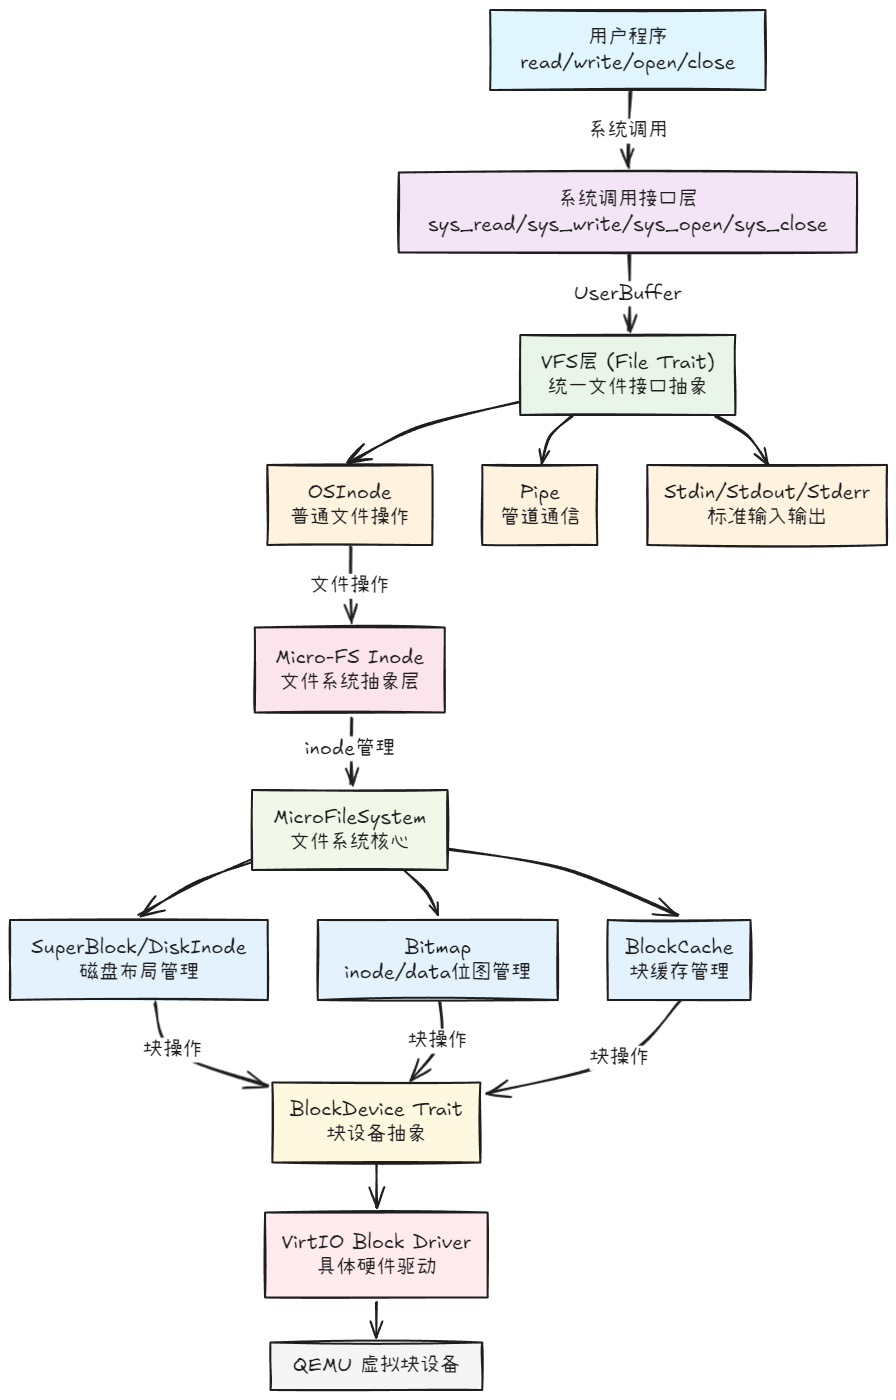
\includegraphics[width=0.8\textwidth]{../image/文件系统.png}
    \caption{文件系统分层架构}
    \label{fig:filesystem-arch}
\end{figure}

\clearpage

\noindent
\rule{0.4\textwidth}{0.4pt}
\hfill
\text{以下为实现介绍}
\hfill
\rule{0.4\textwidth}{0.4pt}

\section{块缓存}

块缓存是文件系统的性能优化核心,它通过在内存中缓存频繁访问的磁盘块来减少实际的磁盘I/O操作。NimlothOS的块缓存采用LRU(最近最少使用)策略,能够有效提高文件系统的读写性能。

\begin{lstlisting}[language=Rust]
pub struct BlockCache {
    cache: [u8; BLOCK_SZ],
    block_id: usize,
    block_device: Arc<dyn BlockDevice>,
    modified: bool,
}

impl BlockCache {
    pub fn sync(&mut self) {
        if self.modified {
            self.modified = false;
            self.block_device.write_block(self.block_id, &self.cache);
        }
    }
}
\end{lstlisting}

每个\texttt{BlockCache}实例代表一个被缓存的磁盘块,包含了512字节的数据缓存、对应的块号、块设备引用以及修改标记。
当缓存中的数据被修改时,系统会设置\texttt{modified}标记,并在适当的时机通过\texttt{sync}方法将数据写回磁盘。
通过这样的延迟写入,可以有效减少磁盘写入次数。

块缓存管理器负责协调多个块缓存的分配和回收,它维护一个固定大小的缓存池,当缓存满时会根据LRU策略替换最久未使用的块。
系统还提供了\texttt{block\_cache\_sync\_all}函数来强制同步所有被修改的缓存到磁盘。

\section{磁盘布局及其数据结构}

\subsection{磁盘布局}

磁盘按照块编号从小到大,可以分成五个区域。第一块是超级块,它用于存放魔数进行文件系统合法性检查,
并存放剩下几个块的位置;第二个区域是索引节点位图,用于记录索引节点是否被使用;第三个区域是索引节点,
用于记录文件的元数据;第四个区域是数据块位图,用于记录数据块是否被使用;第五个区域是数据块,
用于存放文件数据和目录项数据。

\begin{figure}[htbp]
    \centering
    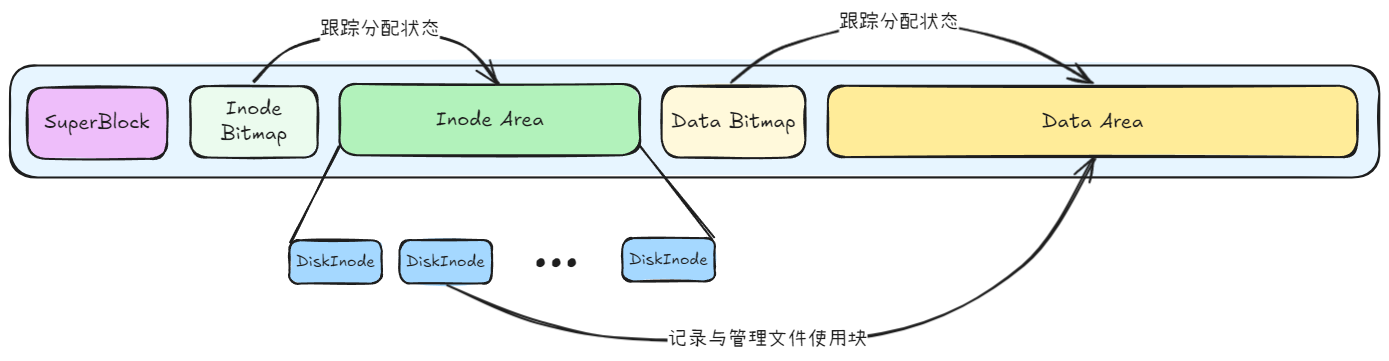
\includegraphics[width=0.8\textwidth]{../image/文件系统磁盘结构.png}
    \caption{磁盘布局}
    \label{fig:disk-layout}
\end{figure}

\subsection{超级块}

超级块存储着整个文件系统的全局信息。它位于磁盘的第0块,包含了文件系统的基本参数和各个区域的布局信息。

\begin{lstlisting}[language=Rust]
#[repr(C)]
pub struct SuperBlock {
    magic: u32,
    pub total_blocks: u32,
    pub inode_bitmap_blocks: u32,
    pub inode_area_blocks: u32,
    pub data_bitmap_blocks: u32,
    pub data_area_blocks: u32,
}

impl SuperBlock {
    pub fn initialize(&mut self, total_blocks: u32, inode_bitmap_blocks: u32,
                     inode_area_blocks: u32, data_bitmap_blocks: u32,
                     data_area_blocks: u32) {
        *self = Self {
            magic: MFS_MAGIC,
            total_blocks, inode_bitmap_blocks, inode_area_blocks,
            data_bitmap_blocks, data_area_blocks,
        }
    }

    pub fn valid(&self) -> bool {
        self.magic == MFS_MAGIC
    }
}
\end{lstlisting}

它通过魔数\texttt{MFS\_MAGIC}来验证文件系统的合法性。其余字段负责记录各个区域占用的块数,当系统启动时,会首先读取超级块来获取整个文件系统的布局信息。

\subsection{位图}

磁盘上有两块位图区域,一块是索引节点位图,一块是数据块位图。位图采用位操作来管理资源的分配状态,每个位对应一个资源单元的使用情况。

\begin{lstlisting}[language=Rust]
pub struct Bitmap {
    start_block_id: usize,
    blocks: usize,
}

impl Bitmap {
    pub fn alloc(&self, block_device: &Arc<dyn BlockDevice>) -> Option<usize> {
        for block_id in 0..self.blocks {
            let pos = block_cache(block_id + self.start_block_id as usize,
                                 Arc::clone(block_device))
                .lock()
                .modify(0, |bitmap_block: &mut BitmapBlock| {
                    if let Some((bits64_pos, inner_pos)) = bitmap_block
                        .iter().enumerate()
                        .find(|(_, bits64)| **bits64 != u64::MAX)
                        .map(|(bits64_pos, bits64)| 
                             (bits64_pos, bits64.trailing_ones() as usize))
                    {
                        bitmap_block[bits64_pos] |= 1u64 << inner_pos;
                        Some(block_id * BLOCK_BITS + bits64_pos * 64 + inner_pos)
                    } else { None }
                });
            if pos.is_some() { return pos; }
        }
        None
    }
}
\end{lstlisting}

位图的实现利用了64位整数的位操作特性,每个\texttt{u64}可以表示64个资源单元的状态。分配算法采用首次适应策略,
从第一个位图块开始查找第一个可用的位。通过\texttt{trailing\_ones}方法能够快速定位到第一个0位。

\subsection{索引节点}

索引节点(inode)是文件系统中每个文件和目录的控制结构,它包含了文件的所有元数据信息以及数据块的索引信息。

\begin{lstlisting}[language=Rust]
#[repr(C)]
pub struct DiskInode {
    pub size: u32,
    pub direct: [u32; INODE_DIRECT_COUNT],
    pub indirect1: u32,
    pub indirect2: u32,
    pub indirect3: u32,
    type_: DiskInodeType,
}

impl DiskInode {
    pub fn block_id(&self, inner_id: u32, 
                   block_device: &Arc<dyn BlockDevice>) -> u32 {
        let inner_id = inner_id as usize;
        if inner_id < INODE_DIRECT_COUNT {
            self.direct[inner_id]
        } else if inner_id < INDIRECT1_BOUND {
            block_cache(self.indirect1 as usize, Arc::clone(block_device))
                .lock()
                .read(0, |indirect_block: &IndirectBlock| {
                    indirect_block[inner_id - INODE_DIRECT_COUNT]
                })
        } else {
            // 处理二级和三级间接块的情况...
        }
    }
}
\end{lstlisting}

inode设计采用了多级索引结构,包含27个直接块索引、一个一级间接块索引、一个二级间接块索引和一个三级间接块索引。这样既能通过直接块高效处理小文件,
又能通过间接块支持大文件。直接块能够快速访问文件的前13.5KB数据,而间接块结构则能够支持最大约1GB的文件大小。

\subsection{数据块}

数据块是文件系统中实际存储文件内容和目录项的区域。每个数据块大小为512字节。数据块的读写操作考虑了跨块访问的情况,
当文件读写操作跨越多个块时,系统会自动处理块边界,确保数据的连续性和完整性。这样使得上层应用可以透明地进行任意大小和位置的文件读写操作。

\section{磁盘块管理器}

磁盘块管理器(BlockManager)是Micro File System的核心组件,它负责管理整个文件系统的状态和操作,包括文件系统的创建、打开、资源分配和回收等功能。

\begin{lstlisting}[language=Rust]
pub struct BlockManager {
    pub block_device: Arc<dyn BlockDevice>,
    pub inode_bitmap: Bitmap,
    pub data_bitmap: Bitmap,
    inode_area_start_block: u32,
    data_area_start_block: u32,
}

impl BlockManager {
    pub fn create(block_device: Arc<dyn BlockDevice>, total_blocks: u32,
                 inode_bitmap_blocks: u32) -> Arc<Mutex<Self>> {
        let inode_bitmap = Bitmap::new(1, inode_bitmap_blocks as usize);
        let inode_num = inode_bitmap.maximum();
        let inode_area_blocks = 
            ((inode_num * core::mem::size_of::<DiskInode>() + BLOCK_SZ - 1) 
             / BLOCK_SZ) as u32;
        
        // 创建文件系统实例并初始化所有数据结构
        let mut mfs = Self {
            block_device: Arc::clone(&block_device),
            inode_bitmap,
            data_bitmap: Bitmap::new((1 + inode_total_blocks) as usize,
                                   data_bitmap_blocks as usize),
            inode_area_start_block: 1 + inode_bitmap_blocks,
            data_area_start_block: 1 + inode_total_blocks + data_bitmap_blocks,
        };
        
        // 初始化根目录
        assert_eq!(mfs.alloc_inode(), 0);
        Arc::new(Mutex::new(mfs))
    }
}
\end{lstlisting}

磁盘块管理器的创建过程如上。它首先根据指定的参数计算各个区域的大小和位置,然后清空所有数据块,创建超级块,最后初始化根目录inode。
这个过程确保了文件系统从一开始就处于一致和可用的状态。根目录的inode号固定为0,使得系统能够快速定位到文件系统的入口点。

磁盘块管理器还提供了资源分配和回收的功能,包括inode分配、数据块分配以及对应的释放操作。这些操作都通过位图来管理,
确保资源分配的高效性和一致性。

\section{Inode文件管理器}

Inode文件管理器提供了文件系统的抽象接口,它封装了底层磁盘inode的复杂性,为上层提供了简洁易用的文件操作API。

\begin{lstlisting}[language=Rust]
pub struct Inode {
    block_id: usize,
    block_offset: usize,
    fs: Arc<Mutex<BlockManager>>,
    block_device: Arc<dyn BlockDevice>,
}

impl Inode {
    pub fn find(&self, path: &str) -> Option<Arc<Inode>> {
        let fs = self.fs.lock();
        let mut block_id = self.block_id as u32;
        let mut block_offset = self.block_offset;
        for name in path.split('/').filter(|s| !s.is_empty()) {
            let inode_id = block_cache(block_id as usize, self.block_device.clone())
                .lock()
                .read(block_offset, |disk_inode: &DiskInode| {
                    if disk_inode.file() { return None; }
                    self.find_inode_id(name, disk_inode)
                });
            if inode_id.is_none() { return None; }
            (block_id, block_offset) = fs.disk_inode_pos(inode_id.unwrap());
        }
        Some(Arc::new(Self::new(block_id, block_offset, 
                               self.fs.clone(), self.block_device.clone())))
    }

    pub fn create(&self, name: &str) -> Option<Arc<Inode>> {
        self.create_inode(name, DiskInodeType::File)
    }
}
\end{lstlisting}

Inode文件管理器将复杂的磁盘操作隐藏在简洁的接口后面。\texttt{find}方法支持路径查找,能够从当前目录开始逐级查找到目标文件或目录。文件创建操作通过\texttt{create}方法实现,它会在当前目录中分配新的inode并添加相应的目录项。

这一层的设计使得文件系统具有了面向对象的特性,每个Inode对象都代表一个具体的文件或目录,用户可以通过这些对象进行各种文件操作,如读写、创建子文件、列出目录内容等。

\section{OSInode}

OSInode是操作系统级别的文件抽象层,它在Inode文件管理器的基础上增加了进程相关的文件操作语义,如文件偏移量管理和权限控制。

\begin{lstlisting}[language=Rust]
pub struct OSInode {
    readable: bool,
    writable: bool,
    inner: UPSafeCell<OSInodeInner>,
}

pub struct OSInodeInner {
    offset: usize,
    inode: Arc<Inode>,
}

impl File for OSInode {
    fn read(&self, mut buf: UserBuffer) -> usize {
        let mut inner = self.inner.exclusive_access();
        let mut total_read_size = 0usize;
        for slice in buf.buffers.iter_mut() {
            let read_size = inner.inode.read_at(inner.offset, *slice);
            if read_size == 0 { break; }
            inner.offset += read_size;
            total_read_size += read_size;
        }
        total_read_size
    }

    fn write(&self, buf: UserBuffer) -> usize {
        let mut inner = self.inner.exclusive_access();
        let mut total_write_size = 0usize;
        for slice in buf.buffers.iter() {
            let write_size = inner.inode.write_at(inner.offset, *slice);
            assert_eq!(write_size, slice.len());
            inner.offset += write_size;
            total_write_size += write_size;
        }
        total_write_size
    }
}
\end{lstlisting}

OSInode为文件操作引入了进程级别的状态管理。每个OSInode实例都维护着独立的文件偏移量,这使得不同进程或同一进程的不同文件描述符可以独立地访问同一个文件。读写权限控制确保了文件访问的安全性,防止了不当的文件操作。

通过实现File trait,OSInode与系统VFS层的集成,文件也可以像其他系统资源一样被统一管理。这也为进程文件描述符表的实现提供了基础,每个文件描述符实际上就是一个OSInode实例的引用。

\section{基于文件的管道机制}

管道机制是进程间通信的重要手段,NimlothOS实现了基于文件接口的管道,使得管道可以像普通文件一样被操作。

\begin{lstlisting}[language=Rust]
pub struct Pipe {
    readable: bool,
    writable: bool,
    buffer: Arc<UPSafeCell<PipeRingBuffer>>,
}

pub struct PipeRingBuffer {
    arr: [u8; RING_BUFFER_SIZE],
    head: usize,
    tail: usize,
    status: RingBufferStatus,
    write_end: Option<Weak<Pipe>>,
}

impl File for Pipe {
    fn read(&self, buf: UserBuffer) -> usize {
        assert!(self.readable);
        let mut already_read = 0usize;
        loop {
            let mut ring_buffer = self.buffer.exclusive_access();
            let loop_read = ring_buffer.available_read();
            if loop_read == 0 {
                if ring_buffer.all_write_ends_closed() {
                    return already_read;
                }
                drop(ring_buffer);
                suspend_current_and_run_next();
                continue;
            }
            // 从环形缓冲区读取数据...
        }
    }
}

pub fn make_pipe() -> (Arc<Pipe>, Arc<Pipe>) {
    let buffer = Arc::new(unsafe { UPSafeCell::new(PipeRingBuffer::new()) });
    let read_end = Arc::new(Pipe::read_end_with_buffer(buffer.clone()));
    let write_end = Arc::new(Pipe::write_end_with_buffer(buffer.clone()));
    (read_end, write_end)
}
\end{lstlisting}

管道的实现基于环形缓冲区。读端在缓冲区为空时会阻塞等待,写端在缓冲区满时也会阻塞等待,这种阻塞机制通过进程调度器实现,能够有效协调进程间的数据传输。

管道的生命周期管理通过弱引用实现,当所有写端关闭且缓冲区为空时,读端会收到EOF信号。这种设计确保了管道在进程结束或文件描述符关闭时能够正确清理资源。

\section{标准输入输出}

标准输入输出是每个进程必备的基础设施,NimlothOS为每个进程提供了三个标准文件描述符:stdin、stdout和stderr。

\begin{lstlisting}[language=Rust]
pub struct Stdin;
pub struct Stdout;
pub struct Stderr;

impl File for Stdin {
    fn read(&self, mut user_buf: UserBuffer) -> usize {
        assert_eq!(user_buf.len(), 1);
        let mut c: usize;
        loop {
            c = console_getchar();
            if c == 0 {
                suspend_current_and_run_next();
                continue;
            } else { break; }
        }
        let ch = c as u8;
        unsafe {
            user_buf.buffers[0].as_mut_ptr().write_volatile(ch);
        }
        1
    }
}

impl File for Stdout {
    fn write(&self, user_buf: UserBuffer) -> usize {
        for buffer in user_buf.buffers.iter() {
            print!("{}", core::str::from_utf8(*buffer).unwrap());
        }
        user_buf.len()
    }
}
\end{lstlisting}

标准输入的实现采用了阻塞式读取策略,当没有输入数据时会主动让出CPU。标准输出和标准错误都直接输出到控制台,支持UTF-8编码的文本处理。

这些标准设备同样实现了File trait,因此可以与文件系统的其他组件无缝集成。进程在创建时会自动分配这三个标准文件描述符,为应用程序提供统一的I/O接口。

\section{标准I/O重定向}

基于统一的File trait接口,NimlothOS能够轻松实现标准I/O重定向功能。进程可以将标准输入重定向到文件或管道,将标准输出重定向到文件、管道或其他设备。
这都依赖于文件描述符表。由于所有的I/O对象都实现了相同的File trait,因此可以在运行时动态替换文件描述符表中的对象,从而实现各种形式的I/O重定向。
这也为shell命令管道、文件重定向等功能提供了支持。


% 第八章:设备驱动程序
% \include{chapters/ch08-device-drivers}

% 第九章:同步与互斥
% \include{chapters/ch09-synchronization}

% 第十章:系统工具与调试
% \include{chapters/ch10-system-tools}

% 第十一章:用户程序与测试
% \include{chapters/ch11-user-programs}

% 第十二章:性能优化与扩展
% \include{chapters/ch12-optimization}

% 附录
\appendix
% \include{chapters/appendix-a-tools}
\chapter{相关资料}

\begin{itemize}
    \item \textbf{\href{https://gpages.juszkiewicz.com.pl/syscalls-table/syscalls.html}{syscalls-table}}
    \item \textbf{\href{https://rcore-os.github.io/rCore-Tutorial-Book-v3/index.html}{rCore-Tutorial-Book}}
    \item \textbf{\href{https://five-embeddev.com/riscv-priv-isa-manual/Priv-v1.12/supervisor.html#supervisor}{RISC-V Privileged ISA Manual}}
    \item \textbf{\href{https://github.com/riscv-non-isa/riscv-sbi-doc}{RISC-V SBI Specification}}
    \item \textbf{\href{https://github.com/mit-pdos/xv6-public}{xv6-public}}
\end{itemize}

\end{document}